\begin{figure}[H] \centering % Created by tikzDevice version 0.12.4 on 2023-07-25 11:08:55
% !TEX encoding = UTF-8 Unicode
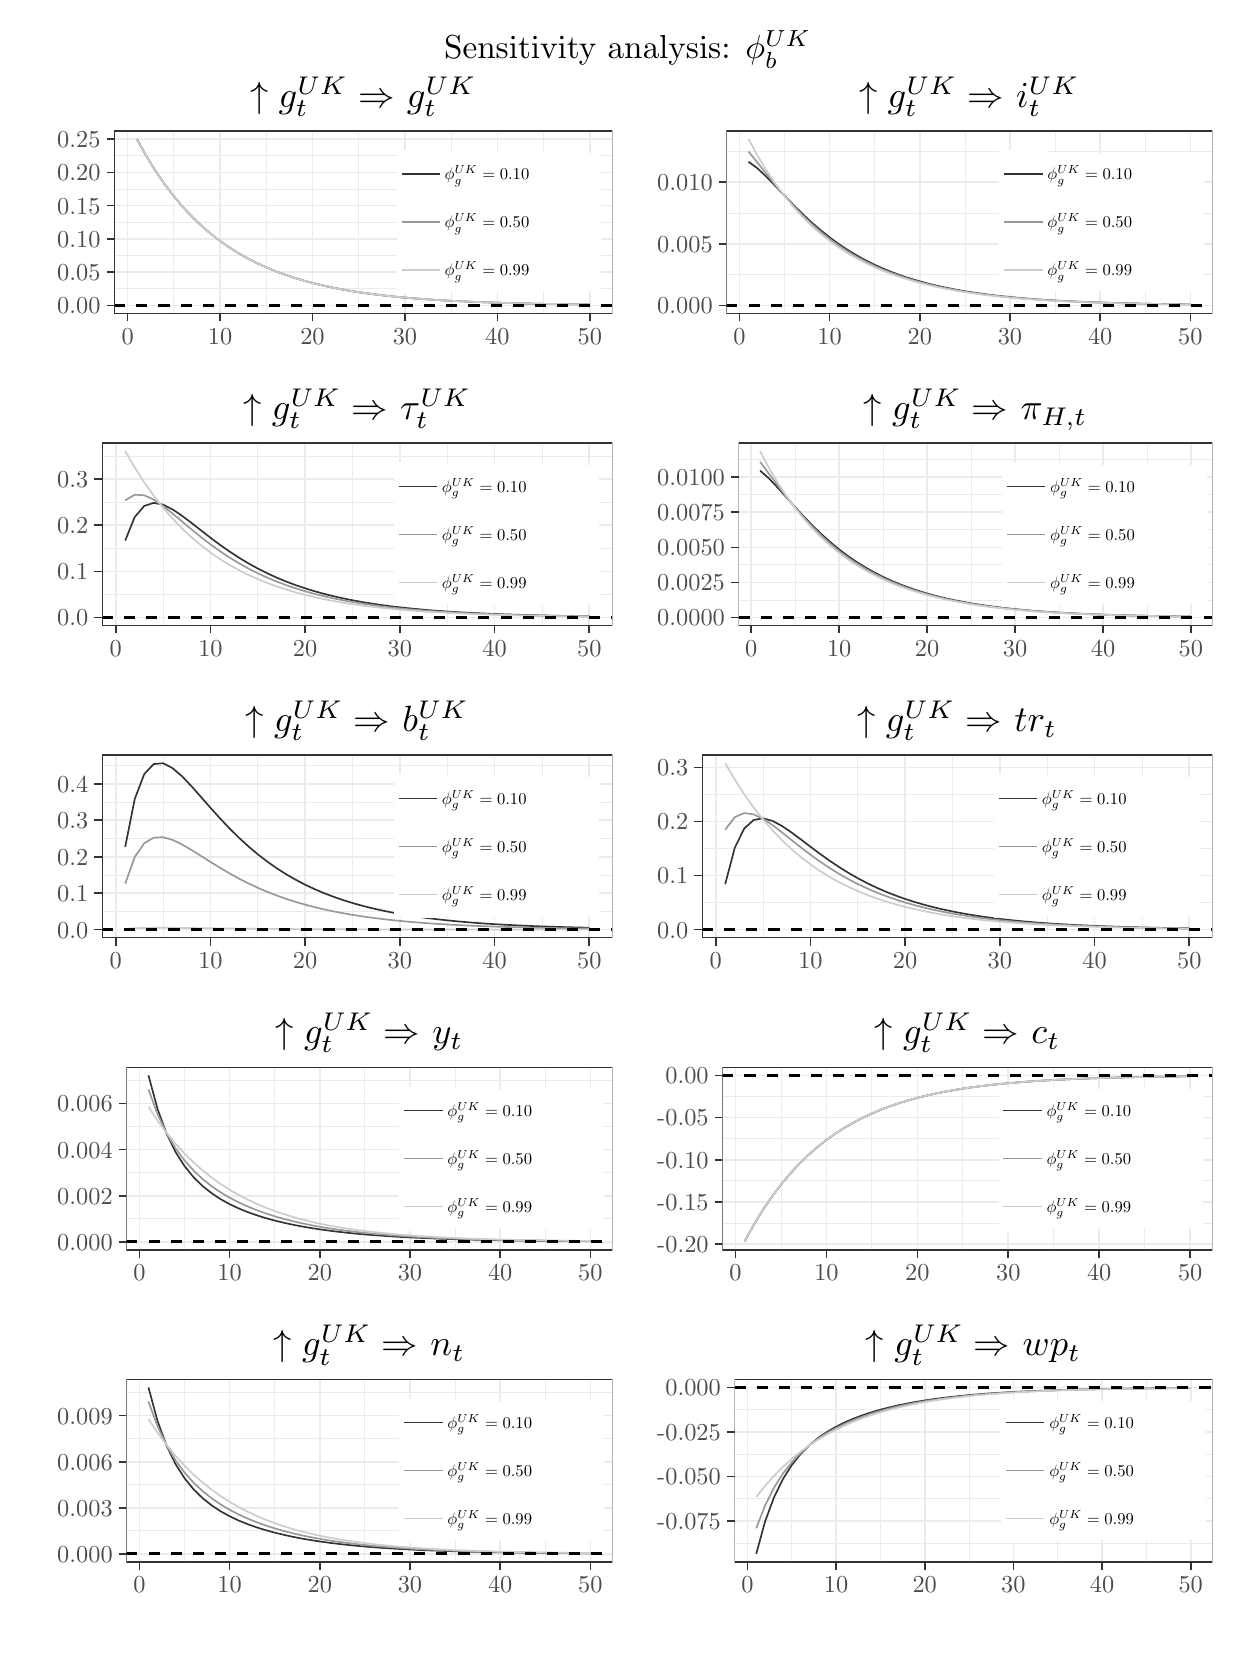
\begin{tikzpicture}[x=1pt,y=1pt]
\definecolor{fillColor}{RGB}{255,255,255}
\path[use as bounding box,fill=fillColor,fill opacity=0.00] (0,0) rectangle (433.62,578.16);
\begin{scope}
\path[clip] (  0.00,451.10) rectangle (216.81,563.87);
\definecolor{drawColor}{RGB}{255,255,255}
\definecolor{fillColor}{RGB}{255,255,255}

\path[draw=drawColor,line width= 0.6pt,line join=round,line cap=round,fill=fillColor] (  0.00,451.10) rectangle (216.81,563.87);
\end{scope}
\begin{scope}
\path[clip] ( 31.27,474.78) rectangle (211.31,540.91);
\definecolor{fillColor}{RGB}{255,255,255}

\path[fill=fillColor] ( 31.27,474.78) rectangle (211.31,540.91);
\definecolor{drawColor}{gray}{0.92}

\path[draw=drawColor,line width= 0.3pt,line join=round] ( 31.27,483.79) --
	(211.31,483.79);

\path[draw=drawColor,line width= 0.3pt,line join=round] ( 31.27,495.82) --
	(211.31,495.82);

\path[draw=drawColor,line width= 0.3pt,line join=round] ( 31.27,507.84) --
	(211.31,507.84);

\path[draw=drawColor,line width= 0.3pt,line join=round] ( 31.27,519.87) --
	(211.31,519.87);

\path[draw=drawColor,line width= 0.3pt,line join=round] ( 31.27,531.89) --
	(211.31,531.89);

\path[draw=drawColor,line width= 0.3pt,line join=round] ( 52.81,474.78) --
	( 52.81,540.91);

\path[draw=drawColor,line width= 0.3pt,line join=round] ( 86.22,474.78) --
	( 86.22,540.91);

\path[draw=drawColor,line width= 0.3pt,line join=round] (119.62,474.78) --
	(119.62,540.91);

\path[draw=drawColor,line width= 0.3pt,line join=round] (153.02,474.78) --
	(153.02,540.91);

\path[draw=drawColor,line width= 0.3pt,line join=round] (186.43,474.78) --
	(186.43,540.91);

\path[draw=drawColor,line width= 0.6pt,line join=round] ( 31.27,477.78) --
	(211.31,477.78);

\path[draw=drawColor,line width= 0.6pt,line join=round] ( 31.27,489.81) --
	(211.31,489.81);

\path[draw=drawColor,line width= 0.6pt,line join=round] ( 31.27,501.83) --
	(211.31,501.83);

\path[draw=drawColor,line width= 0.6pt,line join=round] ( 31.27,513.86) --
	(211.31,513.86);

\path[draw=drawColor,line width= 0.6pt,line join=round] ( 31.27,525.88) --
	(211.31,525.88);

\path[draw=drawColor,line width= 0.6pt,line join=round] ( 31.27,537.90) --
	(211.31,537.90);

\path[draw=drawColor,line width= 0.6pt,line join=round] ( 36.11,474.78) --
	( 36.11,540.91);

\path[draw=drawColor,line width= 0.6pt,line join=round] ( 69.52,474.78) --
	( 69.52,540.91);

\path[draw=drawColor,line width= 0.6pt,line join=round] (102.92,474.78) --
	(102.92,540.91);

\path[draw=drawColor,line width= 0.6pt,line join=round] (136.32,474.78) --
	(136.32,540.91);

\path[draw=drawColor,line width= 0.6pt,line join=round] (169.72,474.78) --
	(169.72,540.91);

\path[draw=drawColor,line width= 0.6pt,line join=round] (203.13,474.78) --
	(203.13,540.91);
\definecolor{drawColor}{gray}{0.20}

\path[draw=drawColor,line width= 0.6pt,line join=round] ( 39.45,537.90) --
	( 42.79,531.89) --
	( 46.13,526.48) --
	( 49.47,521.61) --
	( 52.81,517.23) --
	( 56.15,513.28) --
	( 59.50,509.73) --
	( 62.84,506.54) --
	( 66.18,503.66) --
	( 69.52,501.07) --
	( 72.86,498.75) --
	( 76.20,496.65) --
	( 79.54,494.76) --
	( 82.88,493.06) --
	( 86.22,491.54) --
	( 89.56,490.16) --
	( 92.90,488.92) --
	( 96.24,487.81) --
	( 99.58,486.81) --
	(102.92,485.90) --
	(106.26,485.09) --
	(109.60,484.36) --
	(112.94,483.70) --
	(116.28,483.11) --
	(119.62,482.58) --
	(122.96,482.10) --
	(126.30,481.67) --
	(129.64,481.28) --
	(132.98,480.93) --
	(136.32,480.61) --
	(139.66,480.33) --
	(143.00,480.08) --
	(146.34,479.85) --
	(149.68,479.64) --
	(153.02,479.45) --
	(156.36,479.29) --
	(159.70,479.14) --
	(163.04,479.00) --
	(166.38,478.88) --
	(169.72,478.77) --
	(173.06,478.67) --
	(176.40,478.58) --
	(179.74,478.50) --
	(183.08,478.43) --
	(186.43,478.36) --
	(189.77,478.31) --
	(193.11,478.25) --
	(196.45,478.21) --
	(199.79,478.16) --
	(203.13,478.13);
\definecolor{drawColor}{RGB}{152,152,152}

\path[draw=drawColor,line width= 0.6pt,line join=round] ( 39.45,537.90) --
	( 42.79,531.89) --
	( 46.13,526.48) --
	( 49.47,521.61) --
	( 52.81,517.23) --
	( 56.15,513.28) --
	( 59.50,509.73) --
	( 62.84,506.54) --
	( 66.18,503.66) --
	( 69.52,501.07) --
	( 72.86,498.75) --
	( 76.20,496.65) --
	( 79.54,494.76) --
	( 82.88,493.06) --
	( 86.22,491.54) --
	( 89.56,490.16) --
	( 92.90,488.92) --
	( 96.24,487.81) --
	( 99.58,486.81) --
	(102.92,485.90) --
	(106.26,485.09) --
	(109.60,484.36) --
	(112.94,483.70) --
	(116.28,483.11) --
	(119.62,482.58) --
	(122.96,482.10) --
	(126.30,481.67) --
	(129.64,481.28) --
	(132.98,480.93) --
	(136.32,480.61) --
	(139.66,480.33) --
	(143.00,480.08) --
	(146.34,479.85) --
	(149.68,479.64) --
	(153.02,479.45) --
	(156.36,479.29) --
	(159.70,479.14) --
	(163.04,479.00) --
	(166.38,478.88) --
	(169.72,478.77) --
	(173.06,478.67) --
	(176.40,478.58) --
	(179.74,478.50) --
	(183.08,478.43) --
	(186.43,478.36) --
	(189.77,478.31) --
	(193.11,478.25) --
	(196.45,478.21) --
	(199.79,478.16) --
	(203.13,478.13);
\definecolor{drawColor}{gray}{0.80}

\path[draw=drawColor,line width= 0.6pt,line join=round] ( 39.45,537.90) --
	( 42.79,531.89) --
	( 46.13,526.48) --
	( 49.47,521.61) --
	( 52.81,517.23) --
	( 56.15,513.28) --
	( 59.50,509.73) --
	( 62.84,506.54) --
	( 66.18,503.66) --
	( 69.52,501.07) --
	( 72.86,498.75) --
	( 76.20,496.65) --
	( 79.54,494.76) --
	( 82.88,493.06) --
	( 86.22,491.54) --
	( 89.56,490.16) --
	( 92.90,488.92) --
	( 96.24,487.81) --
	( 99.58,486.81) --
	(102.92,485.90) --
	(106.26,485.09) --
	(109.60,484.36) --
	(112.94,483.70) --
	(116.28,483.11) --
	(119.62,482.58) --
	(122.96,482.10) --
	(126.30,481.67) --
	(129.64,481.28) --
	(132.98,480.93) --
	(136.32,480.61) --
	(139.66,480.33) --
	(143.00,480.08) --
	(146.34,479.85) --
	(149.68,479.64) --
	(153.02,479.45) --
	(156.36,479.29) --
	(159.70,479.14) --
	(163.04,479.00) --
	(166.38,478.88) --
	(169.72,478.77) --
	(173.06,478.67) --
	(176.40,478.58) --
	(179.74,478.50) --
	(183.08,478.43) --
	(186.43,478.36) --
	(189.77,478.31) --
	(193.11,478.25) --
	(196.45,478.21) --
	(199.79,478.16) --
	(203.13,478.13);
\definecolor{drawColor}{RGB}{0,0,0}

\path[draw=drawColor,line width= 1.1pt,dash pattern=on 4pt off 4pt ,line join=round] ( 31.27,477.78) -- (211.31,477.78);
\definecolor{drawColor}{gray}{0.20}

\path[draw=drawColor,line width= 0.6pt,line join=round,line cap=round] ( 31.27,474.78) rectangle (211.31,540.91);
\end{scope}
\begin{scope}
\path[clip] (  0.00,  0.00) rectangle (433.62,578.16);
\definecolor{drawColor}{gray}{0.30}

\node[text=drawColor,anchor=base east,inner sep=0pt, outer sep=0pt, scale=  0.88] at ( 26.32,474.75) {0.00};

\node[text=drawColor,anchor=base east,inner sep=0pt, outer sep=0pt, scale=  0.88] at ( 26.32,486.78) {0.05};

\node[text=drawColor,anchor=base east,inner sep=0pt, outer sep=0pt, scale=  0.88] at ( 26.32,498.80) {0.10};

\node[text=drawColor,anchor=base east,inner sep=0pt, outer sep=0pt, scale=  0.88] at ( 26.32,510.83) {0.15};

\node[text=drawColor,anchor=base east,inner sep=0pt, outer sep=0pt, scale=  0.88] at ( 26.32,522.85) {0.20};

\node[text=drawColor,anchor=base east,inner sep=0pt, outer sep=0pt, scale=  0.88] at ( 26.32,534.87) {0.25};
\end{scope}
\begin{scope}
\path[clip] (  0.00,  0.00) rectangle (433.62,578.16);
\definecolor{drawColor}{gray}{0.20}

\path[draw=drawColor,line width= 0.6pt,line join=round] ( 28.52,477.78) --
	( 31.27,477.78);

\path[draw=drawColor,line width= 0.6pt,line join=round] ( 28.52,489.81) --
	( 31.27,489.81);

\path[draw=drawColor,line width= 0.6pt,line join=round] ( 28.52,501.83) --
	( 31.27,501.83);

\path[draw=drawColor,line width= 0.6pt,line join=round] ( 28.52,513.86) --
	( 31.27,513.86);

\path[draw=drawColor,line width= 0.6pt,line join=round] ( 28.52,525.88) --
	( 31.27,525.88);

\path[draw=drawColor,line width= 0.6pt,line join=round] ( 28.52,537.90) --
	( 31.27,537.90);
\end{scope}
\begin{scope}
\path[clip] (  0.00,  0.00) rectangle (433.62,578.16);
\definecolor{drawColor}{gray}{0.20}

\path[draw=drawColor,line width= 0.6pt,line join=round] ( 36.11,472.03) --
	( 36.11,474.78);

\path[draw=drawColor,line width= 0.6pt,line join=round] ( 69.52,472.03) --
	( 69.52,474.78);

\path[draw=drawColor,line width= 0.6pt,line join=round] (102.92,472.03) --
	(102.92,474.78);

\path[draw=drawColor,line width= 0.6pt,line join=round] (136.32,472.03) --
	(136.32,474.78);

\path[draw=drawColor,line width= 0.6pt,line join=round] (169.72,472.03) --
	(169.72,474.78);

\path[draw=drawColor,line width= 0.6pt,line join=round] (203.13,472.03) --
	(203.13,474.78);
\end{scope}
\begin{scope}
\path[clip] (  0.00,  0.00) rectangle (433.62,578.16);
\definecolor{drawColor}{gray}{0.30}

\node[text=drawColor,anchor=base,inner sep=0pt, outer sep=0pt, scale=  0.88] at ( 36.11,463.76) {0};

\node[text=drawColor,anchor=base,inner sep=0pt, outer sep=0pt, scale=  0.88] at ( 69.52,463.76) {10};

\node[text=drawColor,anchor=base,inner sep=0pt, outer sep=0pt, scale=  0.88] at (102.92,463.76) {20};

\node[text=drawColor,anchor=base,inner sep=0pt, outer sep=0pt, scale=  0.88] at (136.32,463.76) {30};

\node[text=drawColor,anchor=base,inner sep=0pt, outer sep=0pt, scale=  0.88] at (169.72,463.76) {40};

\node[text=drawColor,anchor=base,inner sep=0pt, outer sep=0pt, scale=  0.88] at (203.13,463.76) {50};
\end{scope}
\begin{scope}
\path[clip] (  0.00,  0.00) rectangle (433.62,578.16);
\definecolor{fillColor}{RGB}{255,255,255}

\path[fill=fillColor] (134.34,482.83) rectangle (207.26,532.86);
\end{scope}
\begin{scope}
\path[clip] (  0.00,  0.00) rectangle (433.62,578.16);
\definecolor{fillColor}{RGB}{255,255,255}

\path[fill=fillColor] (133.34,516.52) rectangle (150.69,533.86);
\end{scope}
\begin{scope}
\path[clip] (  0.00,  0.00) rectangle (433.62,578.16);
\definecolor{drawColor}{gray}{0.20}

\path[draw=drawColor,line width= 0.6pt,line join=round] (135.08,525.19) -- (148.95,525.19);
\end{scope}
\begin{scope}
\path[clip] (  0.00,  0.00) rectangle (433.62,578.16);
\definecolor{drawColor}{gray}{0.20}

\path[draw=drawColor,line width= 0.6pt,line join=round] (135.08,525.19) -- (148.95,525.19);
\end{scope}
\begin{scope}
\path[clip] (  0.00,  0.00) rectangle (433.62,578.16);
\definecolor{drawColor}{gray}{0.20}

\path[draw=drawColor,line width= 0.6pt,line join=round] (135.08,525.19) -- (148.95,525.19);
\end{scope}
\begin{scope}
\path[clip] (  0.00,  0.00) rectangle (433.62,578.16);
\definecolor{fillColor}{RGB}{255,255,255}

\path[fill=fillColor] (133.34,499.17) rectangle (150.69,516.52);
\end{scope}
\begin{scope}
\path[clip] (  0.00,  0.00) rectangle (433.62,578.16);
\definecolor{drawColor}{RGB}{152,152,152}

\path[draw=drawColor,line width= 0.6pt,line join=round] (135.08,507.84) -- (148.95,507.84);
\end{scope}
\begin{scope}
\path[clip] (  0.00,  0.00) rectangle (433.62,578.16);
\definecolor{drawColor}{RGB}{152,152,152}

\path[draw=drawColor,line width= 0.6pt,line join=round] (135.08,507.84) -- (148.95,507.84);
\end{scope}
\begin{scope}
\path[clip] (  0.00,  0.00) rectangle (433.62,578.16);
\definecolor{drawColor}{RGB}{152,152,152}

\path[draw=drawColor,line width= 0.6pt,line join=round] (135.08,507.84) -- (148.95,507.84);
\end{scope}
\begin{scope}
\path[clip] (  0.00,  0.00) rectangle (433.62,578.16);
\definecolor{fillColor}{RGB}{255,255,255}

\path[fill=fillColor] (133.34,481.83) rectangle (150.69,499.17);
\end{scope}
\begin{scope}
\path[clip] (  0.00,  0.00) rectangle (433.62,578.16);
\definecolor{drawColor}{gray}{0.80}

\path[draw=drawColor,line width= 0.6pt,line join=round] (135.08,490.50) -- (148.95,490.50);
\end{scope}
\begin{scope}
\path[clip] (  0.00,  0.00) rectangle (433.62,578.16);
\definecolor{drawColor}{gray}{0.80}

\path[draw=drawColor,line width= 0.6pt,line join=round] (135.08,490.50) -- (148.95,490.50);
\end{scope}
\begin{scope}
\path[clip] (  0.00,  0.00) rectangle (433.62,578.16);
\definecolor{drawColor}{gray}{0.80}

\path[draw=drawColor,line width= 0.6pt,line join=round] (135.08,490.50) -- (148.95,490.50);
\end{scope}
\begin{scope}
\path[clip] (  0.00,  0.00) rectangle (433.62,578.16);
\definecolor{drawColor}{RGB}{0,0,0}

\node[text=drawColor,anchor=base west,inner sep=0pt, outer sep=0pt, scale=  0.60] at (150.69,523.12) {${\phi_g^{UK}}=0.10$};
\end{scope}
\begin{scope}
\path[clip] (  0.00,  0.00) rectangle (433.62,578.16);
\definecolor{drawColor}{RGB}{0,0,0}

\node[text=drawColor,anchor=base west,inner sep=0pt, outer sep=0pt, scale=  0.60] at (150.69,505.78) {${\phi_g^{UK}}=0.50$};
\end{scope}
\begin{scope}
\path[clip] (  0.00,  0.00) rectangle (433.62,578.16);
\definecolor{drawColor}{RGB}{0,0,0}

\node[text=drawColor,anchor=base west,inner sep=0pt, outer sep=0pt, scale=  0.60] at (150.69,488.43) {${\phi_g^{UK}}=0.99$};
\end{scope}
\begin{scope}
\path[clip] (  0.00,  0.00) rectangle (433.62,578.16);
\definecolor{drawColor}{RGB}{0,0,0}

\node[text=drawColor,anchor=base,inner sep=0pt, outer sep=0pt, scale=  1.32] at (121.29,549.28) {$\uparrow  g^{UK}_t \Rightarrow $ ${g^{UK}_t}$};
\end{scope}
\begin{scope}
\path[clip] (216.81,451.10) rectangle (433.62,563.87);
\definecolor{drawColor}{RGB}{255,255,255}
\definecolor{fillColor}{RGB}{255,255,255}

\path[draw=drawColor,line width= 0.6pt,line join=round,line cap=round,fill=fillColor] (216.81,451.10) rectangle (433.62,563.87);
\end{scope}
\begin{scope}
\path[clip] (252.48,474.78) rectangle (428.12,540.91);
\definecolor{fillColor}{RGB}{255,255,255}

\path[fill=fillColor] (252.48,474.78) rectangle (428.12,540.91);
\definecolor{drawColor}{gray}{0.92}

\path[draw=drawColor,line width= 0.3pt,line join=round] (252.48,488.93) --
	(428.12,488.93);

\path[draw=drawColor,line width= 0.3pt,line join=round] (252.48,511.21) --
	(428.12,511.21);

\path[draw=drawColor,line width= 0.3pt,line join=round] (252.48,533.50) --
	(428.12,533.50);

\path[draw=drawColor,line width= 0.3pt,line join=round] (273.50,474.78) --
	(273.50,540.91);

\path[draw=drawColor,line width= 0.3pt,line join=round] (306.08,474.78) --
	(306.08,540.91);

\path[draw=drawColor,line width= 0.3pt,line join=round] (338.67,474.78) --
	(338.67,540.91);

\path[draw=drawColor,line width= 0.3pt,line join=round] (371.26,474.78) --
	(371.26,540.91);

\path[draw=drawColor,line width= 0.3pt,line join=round] (403.84,474.78) --
	(403.84,540.91);

\path[draw=drawColor,line width= 0.6pt,line join=round] (252.48,477.78) --
	(428.12,477.78);

\path[draw=drawColor,line width= 0.6pt,line join=round] (252.48,500.07) --
	(428.12,500.07);

\path[draw=drawColor,line width= 0.6pt,line join=round] (252.48,522.36) --
	(428.12,522.36);

\path[draw=drawColor,line width= 0.6pt,line join=round] (257.20,474.78) --
	(257.20,540.91);

\path[draw=drawColor,line width= 0.6pt,line join=round] (289.79,474.78) --
	(289.79,540.91);

\path[draw=drawColor,line width= 0.6pt,line join=round] (322.38,474.78) --
	(322.38,540.91);

\path[draw=drawColor,line width= 0.6pt,line join=round] (354.96,474.78) --
	(354.96,540.91);

\path[draw=drawColor,line width= 0.6pt,line join=round] (387.55,474.78) --
	(387.55,540.91);

\path[draw=drawColor,line width= 0.6pt,line join=round] (420.14,474.78) --
	(420.14,540.91);
\definecolor{drawColor}{gray}{0.20}

\path[draw=drawColor,line width= 0.6pt,line join=round] (260.46,529.71) --
	(263.72,527.31) --
	(266.98,524.25) --
	(270.24,520.88) --
	(273.50,517.44) --
	(276.76,514.06) --
	(280.01,510.83) --
	(283.27,507.79) --
	(286.53,504.97) --
	(289.79,502.38) --
	(293.05,500.00) --
	(296.31,497.83) --
	(299.57,495.87) --
	(302.82,494.08) --
	(306.08,492.47) --
	(309.34,491.01) --
	(312.60,489.70) --
	(315.86,488.51) --
	(319.12,487.44) --
	(322.38,486.48) --
	(325.64,485.61) --
	(328.89,484.83) --
	(332.15,484.13) --
	(335.41,483.49) --
	(338.67,482.92) --
	(341.93,482.41) --
	(345.19,481.95) --
	(348.45,481.53) --
	(351.70,481.15) --
	(354.96,480.82) --
	(358.22,480.51) --
	(361.48,480.24) --
	(364.74,479.99) --
	(368.00,479.77) --
	(371.26,479.57) --
	(374.52,479.39) --
	(377.77,479.23) --
	(381.03,479.09) --
	(384.29,478.96) --
	(387.55,478.84) --
	(390.81,478.73) --
	(394.07,478.64) --
	(397.33,478.55) --
	(400.58,478.48) --
	(403.84,478.41) --
	(407.10,478.34) --
	(410.36,478.29) --
	(413.62,478.24) --
	(416.88,478.19) --
	(420.14,478.15);
\definecolor{drawColor}{RGB}{152,152,152}

\path[draw=drawColor,line width= 0.6pt,line join=round] (260.46,533.39) --
	(263.72,529.39) --
	(266.98,525.28) --
	(270.24,521.24) --
	(273.50,517.37) --
	(276.76,513.74) --
	(280.01,510.36) --
	(283.27,507.25) --
	(286.53,504.41) --
	(289.79,501.81) --
	(293.05,499.46) --
	(296.31,497.32) --
	(299.57,495.39) --
	(302.82,493.64) --
	(306.08,492.07) --
	(309.34,490.64) --
	(312.60,489.36) --
	(315.86,488.21) --
	(319.12,487.17) --
	(322.38,486.23) --
	(325.64,485.39) --
	(328.89,484.63) --
	(332.15,483.94) --
	(335.41,483.33) --
	(338.67,482.77) --
	(341.93,482.27) --
	(345.19,481.82) --
	(348.45,481.42) --
	(351.70,481.06) --
	(354.96,480.73) --
	(358.22,480.43) --
	(361.48,480.17) --
	(364.74,479.93) --
	(368.00,479.72) --
	(371.26,479.52) --
	(374.52,479.35) --
	(377.77,479.19) --
	(381.03,479.05) --
	(384.29,478.92) --
	(387.55,478.81) --
	(390.81,478.71) --
	(394.07,478.61) --
	(397.33,478.53) --
	(400.58,478.46) --
	(403.84,478.39) --
	(407.10,478.33) --
	(410.36,478.27) --
	(413.62,478.22) --
	(416.88,478.18) --
	(420.14,478.14);
\definecolor{drawColor}{gray}{0.80}

\path[draw=drawColor,line width= 0.6pt,line join=round] (260.46,537.90) --
	(263.72,531.93) --
	(266.98,526.53) --
	(270.24,521.67) --
	(273.50,517.29) --
	(276.76,513.35) --
	(280.01,509.80) --
	(283.27,506.60) --
	(286.53,503.72) --
	(289.79,501.13) --
	(293.05,498.79) --
	(296.31,496.69) --
	(299.57,494.80) --
	(302.82,493.10) --
	(306.08,491.57) --
	(309.34,490.19) --
	(312.60,488.95) --
	(315.86,487.83) --
	(319.12,486.83) --
	(322.38,485.92) --
	(325.64,485.11) --
	(328.89,484.38) --
	(332.15,483.72) --
	(335.41,483.12) --
	(338.67,482.59) --
	(341.93,482.11) --
	(345.19,481.68) --
	(348.45,481.29) --
	(351.70,480.94) --
	(354.96,480.62) --
	(358.22,480.34) --
	(361.48,480.08) --
	(364.74,479.85) --
	(368.00,479.64) --
	(371.26,479.46) --
	(374.52,479.29) --
	(377.77,479.14) --
	(381.03,479.00) --
	(384.29,478.88) --
	(387.55,478.77) --
	(390.81,478.67) --
	(394.07,478.58) --
	(397.33,478.50) --
	(400.58,478.43) --
	(403.84,478.37) --
	(407.10,478.31) --
	(410.36,478.26) --
	(413.62,478.21) --
	(416.88,478.17) --
	(420.14,478.13);
\definecolor{drawColor}{RGB}{0,0,0}

\path[draw=drawColor,line width= 1.1pt,dash pattern=on 4pt off 4pt ,line join=round] (252.48,477.78) -- (428.12,477.78);
\definecolor{drawColor}{gray}{0.20}

\path[draw=drawColor,line width= 0.6pt,line join=round,line cap=round] (252.48,474.78) rectangle (428.12,540.91);
\end{scope}
\begin{scope}
\path[clip] (  0.00,  0.00) rectangle (433.62,578.16);
\definecolor{drawColor}{gray}{0.30}

\node[text=drawColor,anchor=base east,inner sep=0pt, outer sep=0pt, scale=  0.88] at (247.53,474.75) {0.000};

\node[text=drawColor,anchor=base east,inner sep=0pt, outer sep=0pt, scale=  0.88] at (247.53,497.04) {0.005};

\node[text=drawColor,anchor=base east,inner sep=0pt, outer sep=0pt, scale=  0.88] at (247.53,519.33) {0.010};
\end{scope}
\begin{scope}
\path[clip] (  0.00,  0.00) rectangle (433.62,578.16);
\definecolor{drawColor}{gray}{0.20}

\path[draw=drawColor,line width= 0.6pt,line join=round] (249.73,477.78) --
	(252.48,477.78);

\path[draw=drawColor,line width= 0.6pt,line join=round] (249.73,500.07) --
	(252.48,500.07);

\path[draw=drawColor,line width= 0.6pt,line join=round] (249.73,522.36) --
	(252.48,522.36);
\end{scope}
\begin{scope}
\path[clip] (  0.00,  0.00) rectangle (433.62,578.16);
\definecolor{drawColor}{gray}{0.20}

\path[draw=drawColor,line width= 0.6pt,line join=round] (257.20,472.03) --
	(257.20,474.78);

\path[draw=drawColor,line width= 0.6pt,line join=round] (289.79,472.03) --
	(289.79,474.78);

\path[draw=drawColor,line width= 0.6pt,line join=round] (322.38,472.03) --
	(322.38,474.78);

\path[draw=drawColor,line width= 0.6pt,line join=round] (354.96,472.03) --
	(354.96,474.78);

\path[draw=drawColor,line width= 0.6pt,line join=round] (387.55,472.03) --
	(387.55,474.78);

\path[draw=drawColor,line width= 0.6pt,line join=round] (420.14,472.03) --
	(420.14,474.78);
\end{scope}
\begin{scope}
\path[clip] (  0.00,  0.00) rectangle (433.62,578.16);
\definecolor{drawColor}{gray}{0.30}

\node[text=drawColor,anchor=base,inner sep=0pt, outer sep=0pt, scale=  0.88] at (257.20,463.76) {0};

\node[text=drawColor,anchor=base,inner sep=0pt, outer sep=0pt, scale=  0.88] at (289.79,463.76) {10};

\node[text=drawColor,anchor=base,inner sep=0pt, outer sep=0pt, scale=  0.88] at (322.38,463.76) {20};

\node[text=drawColor,anchor=base,inner sep=0pt, outer sep=0pt, scale=  0.88] at (354.96,463.76) {30};

\node[text=drawColor,anchor=base,inner sep=0pt, outer sep=0pt, scale=  0.88] at (387.55,463.76) {40};

\node[text=drawColor,anchor=base,inner sep=0pt, outer sep=0pt, scale=  0.88] at (420.14,463.76) {50};
\end{scope}
\begin{scope}
\path[clip] (  0.00,  0.00) rectangle (433.62,578.16);
\definecolor{fillColor}{RGB}{255,255,255}

\path[fill=fillColor] (352.14,482.83) rectangle (425.06,532.86);
\end{scope}
\begin{scope}
\path[clip] (  0.00,  0.00) rectangle (433.62,578.16);
\definecolor{fillColor}{RGB}{255,255,255}

\path[fill=fillColor] (351.14,516.52) rectangle (368.49,533.86);
\end{scope}
\begin{scope}
\path[clip] (  0.00,  0.00) rectangle (433.62,578.16);
\definecolor{drawColor}{gray}{0.20}

\path[draw=drawColor,line width= 0.6pt,line join=round] (352.88,525.19) -- (366.75,525.19);
\end{scope}
\begin{scope}
\path[clip] (  0.00,  0.00) rectangle (433.62,578.16);
\definecolor{drawColor}{gray}{0.20}

\path[draw=drawColor,line width= 0.6pt,line join=round] (352.88,525.19) -- (366.75,525.19);
\end{scope}
\begin{scope}
\path[clip] (  0.00,  0.00) rectangle (433.62,578.16);
\definecolor{drawColor}{gray}{0.20}

\path[draw=drawColor,line width= 0.6pt,line join=round] (352.88,525.19) -- (366.75,525.19);
\end{scope}
\begin{scope}
\path[clip] (  0.00,  0.00) rectangle (433.62,578.16);
\definecolor{fillColor}{RGB}{255,255,255}

\path[fill=fillColor] (351.14,499.17) rectangle (368.49,516.52);
\end{scope}
\begin{scope}
\path[clip] (  0.00,  0.00) rectangle (433.62,578.16);
\definecolor{drawColor}{RGB}{152,152,152}

\path[draw=drawColor,line width= 0.6pt,line join=round] (352.88,507.84) -- (366.75,507.84);
\end{scope}
\begin{scope}
\path[clip] (  0.00,  0.00) rectangle (433.62,578.16);
\definecolor{drawColor}{RGB}{152,152,152}

\path[draw=drawColor,line width= 0.6pt,line join=round] (352.88,507.84) -- (366.75,507.84);
\end{scope}
\begin{scope}
\path[clip] (  0.00,  0.00) rectangle (433.62,578.16);
\definecolor{drawColor}{RGB}{152,152,152}

\path[draw=drawColor,line width= 0.6pt,line join=round] (352.88,507.84) -- (366.75,507.84);
\end{scope}
\begin{scope}
\path[clip] (  0.00,  0.00) rectangle (433.62,578.16);
\definecolor{fillColor}{RGB}{255,255,255}

\path[fill=fillColor] (351.14,481.83) rectangle (368.49,499.17);
\end{scope}
\begin{scope}
\path[clip] (  0.00,  0.00) rectangle (433.62,578.16);
\definecolor{drawColor}{gray}{0.80}

\path[draw=drawColor,line width= 0.6pt,line join=round] (352.88,490.50) -- (366.75,490.50);
\end{scope}
\begin{scope}
\path[clip] (  0.00,  0.00) rectangle (433.62,578.16);
\definecolor{drawColor}{gray}{0.80}

\path[draw=drawColor,line width= 0.6pt,line join=round] (352.88,490.50) -- (366.75,490.50);
\end{scope}
\begin{scope}
\path[clip] (  0.00,  0.00) rectangle (433.62,578.16);
\definecolor{drawColor}{gray}{0.80}

\path[draw=drawColor,line width= 0.6pt,line join=round] (352.88,490.50) -- (366.75,490.50);
\end{scope}
\begin{scope}
\path[clip] (  0.00,  0.00) rectangle (433.62,578.16);
\definecolor{drawColor}{RGB}{0,0,0}

\node[text=drawColor,anchor=base west,inner sep=0pt, outer sep=0pt, scale=  0.60] at (368.49,523.12) {${\phi_g^{UK}}=0.10$};
\end{scope}
\begin{scope}
\path[clip] (  0.00,  0.00) rectangle (433.62,578.16);
\definecolor{drawColor}{RGB}{0,0,0}

\node[text=drawColor,anchor=base west,inner sep=0pt, outer sep=0pt, scale=  0.60] at (368.49,505.78) {${\phi_g^{UK}}=0.50$};
\end{scope}
\begin{scope}
\path[clip] (  0.00,  0.00) rectangle (433.62,578.16);
\definecolor{drawColor}{RGB}{0,0,0}

\node[text=drawColor,anchor=base west,inner sep=0pt, outer sep=0pt, scale=  0.60] at (368.49,488.43) {${\phi_g^{UK}}=0.99$};
\end{scope}
\begin{scope}
\path[clip] (  0.00,  0.00) rectangle (433.62,578.16);
\definecolor{drawColor}{RGB}{0,0,0}

\node[text=drawColor,anchor=base,inner sep=0pt, outer sep=0pt, scale=  1.32] at (340.30,549.28) {$\uparrow  g^{UK}_t \Rightarrow $ ${i^{UK}_t}$};
\end{scope}
\begin{scope}
\path[clip] (  0.00,338.32) rectangle (216.81,451.10);
\definecolor{drawColor}{RGB}{255,255,255}
\definecolor{fillColor}{RGB}{255,255,255}

\path[draw=drawColor,line width= 0.6pt,line join=round,line cap=round,fill=fillColor] (  0.00,338.32) rectangle (216.81,451.10);
\end{scope}
\begin{scope}
\path[clip] ( 26.87,362.00) rectangle (211.31,428.14);
\definecolor{fillColor}{RGB}{255,255,255}

\path[fill=fillColor] ( 26.87,362.00) rectangle (211.31,428.14);
\definecolor{drawColor}{gray}{0.92}

\path[draw=drawColor,line width= 0.3pt,line join=round] ( 26.87,373.34) --
	(211.31,373.34);

\path[draw=drawColor,line width= 0.3pt,line join=round] ( 26.87,390.01) --
	(211.31,390.01);

\path[draw=drawColor,line width= 0.3pt,line join=round] ( 26.87,406.69) --
	(211.31,406.69);

\path[draw=drawColor,line width= 0.3pt,line join=round] ( 26.87,423.36) --
	(211.31,423.36);

\path[draw=drawColor,line width= 0.3pt,line join=round] ( 48.94,362.00) --
	( 48.94,428.14);

\path[draw=drawColor,line width= 0.3pt,line join=round] ( 83.16,362.00) --
	( 83.16,428.14);

\path[draw=drawColor,line width= 0.3pt,line join=round] (117.38,362.00) --
	(117.38,428.14);

\path[draw=drawColor,line width= 0.3pt,line join=round] (151.60,362.00) --
	(151.60,428.14);

\path[draw=drawColor,line width= 0.3pt,line join=round] (185.82,362.00) --
	(185.82,428.14);

\path[draw=drawColor,line width= 0.6pt,line join=round] ( 26.87,365.01) --
	(211.31,365.01);

\path[draw=drawColor,line width= 0.6pt,line join=round] ( 26.87,381.68) --
	(211.31,381.68);

\path[draw=drawColor,line width= 0.6pt,line join=round] ( 26.87,398.35) --
	(211.31,398.35);

\path[draw=drawColor,line width= 0.6pt,line join=round] ( 26.87,415.02) --
	(211.31,415.02);

\path[draw=drawColor,line width= 0.6pt,line join=round] ( 31.83,362.00) --
	( 31.83,428.14);

\path[draw=drawColor,line width= 0.6pt,line join=round] ( 66.05,362.00) --
	( 66.05,428.14);

\path[draw=drawColor,line width= 0.6pt,line join=round] (100.27,362.00) --
	(100.27,428.14);

\path[draw=drawColor,line width= 0.6pt,line join=round] (134.49,362.00) --
	(134.49,428.14);

\path[draw=drawColor,line width= 0.6pt,line join=round] (168.71,362.00) --
	(168.71,428.14);

\path[draw=drawColor,line width= 0.6pt,line join=round] (202.93,362.00) --
	(202.93,428.14);
\definecolor{drawColor}{gray}{0.20}

\path[draw=drawColor,line width= 0.6pt,line join=round] ( 35.25,392.83) --
	( 38.68,401.32) --
	( 42.10,405.32) --
	( 45.52,406.45) --
	( 48.94,405.80) --
	( 52.36,404.09) --
	( 55.79,401.78) --
	( 59.21,399.19) --
	( 62.63,396.50) --
	( 66.05,393.85) --
	( 69.47,391.30) --
	( 72.90,388.90) --
	( 76.32,386.66) --
	( 79.74,384.60) --
	( 83.16,382.71) --
	( 86.58,380.99) --
	( 90.00,379.42) --
	( 93.43,378.00) --
	( 96.85,376.72) --
	(100.27,375.56) --
	(103.69,374.51) --
	(107.11,373.56) --
	(110.54,372.71) --
	(113.96,371.94) --
	(117.38,371.25) --
	(120.80,370.63) --
	(124.22,370.07) --
	(127.65,369.56) --
	(131.07,369.11) --
	(134.49,368.70) --
	(137.91,368.33) --
	(141.33,368.00) --
	(144.75,367.70) --
	(148.18,367.43) --
	(151.60,367.19) --
	(155.02,366.97) --
	(158.44,366.77) --
	(161.86,366.60) --
	(165.29,366.44) --
	(168.71,366.29) --
	(172.13,366.16) --
	(175.55,366.05) --
	(178.97,365.94) --
	(182.40,365.85) --
	(185.82,365.77) --
	(189.24,365.69) --
	(192.66,365.62) --
	(196.08,365.56) --
	(199.50,365.51) --
	(202.93,365.46);
\definecolor{drawColor}{RGB}{152,152,152}

\path[draw=drawColor,line width= 0.6pt,line join=round] ( 35.25,407.35) --
	( 38.68,409.38) --
	( 42.10,409.18) --
	( 45.52,407.63) --
	( 48.94,405.31) --
	( 52.36,402.59) --
	( 55.79,399.72) --
	( 59.21,396.85) --
	( 62.63,394.08) --
	( 66.05,391.45) --
	( 69.47,388.99) --
	( 72.90,386.72) --
	( 76.32,384.63) --
	( 79.74,382.73) --
	( 83.16,380.99) --
	( 86.58,379.42) --
	( 90.00,378.00) --
	( 93.43,376.71) --
	( 96.85,375.55) --
	(100.27,374.50) --
	(103.69,373.55) --
	(107.11,372.70) --
	(110.54,371.93) --
	(113.96,371.24) --
	(117.38,370.62) --
	(120.80,370.06) --
	(124.22,369.55) --
	(127.65,369.10) --
	(131.07,368.69) --
	(134.49,368.32) --
	(137.91,367.99) --
	(141.33,367.69) --
	(144.75,367.42) --
	(148.18,367.18) --
	(151.60,366.97) --
	(155.02,366.77) --
	(158.44,366.59) --
	(161.86,366.43) --
	(165.29,366.29) --
	(168.71,366.16) --
	(172.13,366.05) --
	(175.55,365.94) --
	(178.97,365.85) --
	(182.40,365.77) --
	(185.82,365.69) --
	(189.24,365.62) --
	(192.66,365.56) --
	(196.08,365.50) --
	(199.50,365.46) --
	(202.93,365.41);
\definecolor{drawColor}{gray}{0.80}

\path[draw=drawColor,line width= 0.6pt,line join=round] ( 35.25,425.13) --
	( 38.68,419.24) --
	( 42.10,413.90) --
	( 45.52,409.07) --
	( 48.94,404.70) --
	( 52.36,400.76) --
	( 55.79,397.20) --
	( 59.21,394.00) --
	( 62.63,391.11) --
	( 66.05,388.50) --
	( 69.47,386.16) --
	( 72.90,384.04) --
	( 76.32,382.14) --
	( 79.74,380.43) --
	( 83.16,378.89) --
	( 86.58,377.50) --
	( 90.00,376.25) --
	( 93.43,375.13) --
	( 96.85,374.12) --
	(100.27,373.20) --
	(103.69,372.38) --
	(107.11,371.65) --
	(110.54,370.98) --
	(113.96,370.39) --
	(117.38,369.85) --
	(120.80,369.36) --
	(124.22,368.93) --
	(127.65,368.54) --
	(131.07,368.18) --
	(134.49,367.87) --
	(137.91,367.58) --
	(141.33,367.32) --
	(144.75,367.09) --
	(148.18,366.88) --
	(151.60,366.70) --
	(155.02,366.53) --
	(158.44,366.37) --
	(161.86,366.24) --
	(165.29,366.11) --
	(168.71,366.00) --
	(172.13,365.90) --
	(175.55,365.81) --
	(178.97,365.73) --
	(182.40,365.66) --
	(185.82,365.60) --
	(189.24,365.54) --
	(192.66,365.48) --
	(196.08,365.44) --
	(199.50,365.39) --
	(202.93,365.35);
\definecolor{drawColor}{RGB}{0,0,0}

\path[draw=drawColor,line width= 1.1pt,dash pattern=on 4pt off 4pt ,line join=round] ( 26.87,365.01) -- (211.31,365.01);
\definecolor{drawColor}{gray}{0.20}

\path[draw=drawColor,line width= 0.6pt,line join=round,line cap=round] ( 26.87,362.00) rectangle (211.31,428.14);
\end{scope}
\begin{scope}
\path[clip] (  0.00,  0.00) rectangle (433.62,578.16);
\definecolor{drawColor}{gray}{0.30}

\node[text=drawColor,anchor=base east,inner sep=0pt, outer sep=0pt, scale=  0.88] at ( 21.92,361.98) {0.0};

\node[text=drawColor,anchor=base east,inner sep=0pt, outer sep=0pt, scale=  0.88] at ( 21.92,378.65) {0.1};

\node[text=drawColor,anchor=base east,inner sep=0pt, outer sep=0pt, scale=  0.88] at ( 21.92,395.32) {0.2};

\node[text=drawColor,anchor=base east,inner sep=0pt, outer sep=0pt, scale=  0.88] at ( 21.92,411.99) {0.3};
\end{scope}
\begin{scope}
\path[clip] (  0.00,  0.00) rectangle (433.62,578.16);
\definecolor{drawColor}{gray}{0.20}

\path[draw=drawColor,line width= 0.6pt,line join=round] ( 24.12,365.01) --
	( 26.87,365.01);

\path[draw=drawColor,line width= 0.6pt,line join=round] ( 24.12,381.68) --
	( 26.87,381.68);

\path[draw=drawColor,line width= 0.6pt,line join=round] ( 24.12,398.35) --
	( 26.87,398.35);

\path[draw=drawColor,line width= 0.6pt,line join=round] ( 24.12,415.02) --
	( 26.87,415.02);
\end{scope}
\begin{scope}
\path[clip] (  0.00,  0.00) rectangle (433.62,578.16);
\definecolor{drawColor}{gray}{0.20}

\path[draw=drawColor,line width= 0.6pt,line join=round] ( 31.83,359.25) --
	( 31.83,362.00);

\path[draw=drawColor,line width= 0.6pt,line join=round] ( 66.05,359.25) --
	( 66.05,362.00);

\path[draw=drawColor,line width= 0.6pt,line join=round] (100.27,359.25) --
	(100.27,362.00);

\path[draw=drawColor,line width= 0.6pt,line join=round] (134.49,359.25) --
	(134.49,362.00);

\path[draw=drawColor,line width= 0.6pt,line join=round] (168.71,359.25) --
	(168.71,362.00);

\path[draw=drawColor,line width= 0.6pt,line join=round] (202.93,359.25) --
	(202.93,362.00);
\end{scope}
\begin{scope}
\path[clip] (  0.00,  0.00) rectangle (433.62,578.16);
\definecolor{drawColor}{gray}{0.30}

\node[text=drawColor,anchor=base,inner sep=0pt, outer sep=0pt, scale=  0.88] at ( 31.83,350.99) {0};

\node[text=drawColor,anchor=base,inner sep=0pt, outer sep=0pt, scale=  0.88] at ( 66.05,350.99) {10};

\node[text=drawColor,anchor=base,inner sep=0pt, outer sep=0pt, scale=  0.88] at (100.27,350.99) {20};

\node[text=drawColor,anchor=base,inner sep=0pt, outer sep=0pt, scale=  0.88] at (134.49,350.99) {30};

\node[text=drawColor,anchor=base,inner sep=0pt, outer sep=0pt, scale=  0.88] at (168.71,350.99) {40};

\node[text=drawColor,anchor=base,inner sep=0pt, outer sep=0pt, scale=  0.88] at (202.93,350.99) {50};
\end{scope}
\begin{scope}
\path[clip] (  0.00,  0.00) rectangle (433.62,578.16);
\definecolor{fillColor}{RGB}{255,255,255}

\path[fill=fillColor] (133.35,370.05) rectangle (206.27,420.09);
\end{scope}
\begin{scope}
\path[clip] (  0.00,  0.00) rectangle (433.62,578.16);
\definecolor{fillColor}{RGB}{255,255,255}

\path[fill=fillColor] (132.35,403.74) rectangle (149.70,421.09);
\end{scope}
\begin{scope}
\path[clip] (  0.00,  0.00) rectangle (433.62,578.16);
\definecolor{drawColor}{gray}{0.20}

\path[draw=drawColor,line width= 0.6pt,line join=round] (134.09,412.41) -- (147.96,412.41);
\end{scope}
\begin{scope}
\path[clip] (  0.00,  0.00) rectangle (433.62,578.16);
\definecolor{drawColor}{gray}{0.20}

\path[draw=drawColor,line width= 0.6pt,line join=round] (134.09,412.41) -- (147.96,412.41);
\end{scope}
\begin{scope}
\path[clip] (  0.00,  0.00) rectangle (433.62,578.16);
\definecolor{drawColor}{gray}{0.20}

\path[draw=drawColor,line width= 0.6pt,line join=round] (134.09,412.41) -- (147.96,412.41);
\end{scope}
\begin{scope}
\path[clip] (  0.00,  0.00) rectangle (433.62,578.16);
\definecolor{fillColor}{RGB}{255,255,255}

\path[fill=fillColor] (132.35,386.40) rectangle (149.70,403.74);
\end{scope}
\begin{scope}
\path[clip] (  0.00,  0.00) rectangle (433.62,578.16);
\definecolor{drawColor}{RGB}{152,152,152}

\path[draw=drawColor,line width= 0.6pt,line join=round] (134.09,395.07) -- (147.96,395.07);
\end{scope}
\begin{scope}
\path[clip] (  0.00,  0.00) rectangle (433.62,578.16);
\definecolor{drawColor}{RGB}{152,152,152}

\path[draw=drawColor,line width= 0.6pt,line join=round] (134.09,395.07) -- (147.96,395.07);
\end{scope}
\begin{scope}
\path[clip] (  0.00,  0.00) rectangle (433.62,578.16);
\definecolor{drawColor}{RGB}{152,152,152}

\path[draw=drawColor,line width= 0.6pt,line join=round] (134.09,395.07) -- (147.96,395.07);
\end{scope}
\begin{scope}
\path[clip] (  0.00,  0.00) rectangle (433.62,578.16);
\definecolor{fillColor}{RGB}{255,255,255}

\path[fill=fillColor] (132.35,369.05) rectangle (149.70,386.40);
\end{scope}
\begin{scope}
\path[clip] (  0.00,  0.00) rectangle (433.62,578.16);
\definecolor{drawColor}{gray}{0.80}

\path[draw=drawColor,line width= 0.6pt,line join=round] (134.09,377.72) -- (147.96,377.72);
\end{scope}
\begin{scope}
\path[clip] (  0.00,  0.00) rectangle (433.62,578.16);
\definecolor{drawColor}{gray}{0.80}

\path[draw=drawColor,line width= 0.6pt,line join=round] (134.09,377.72) -- (147.96,377.72);
\end{scope}
\begin{scope}
\path[clip] (  0.00,  0.00) rectangle (433.62,578.16);
\definecolor{drawColor}{gray}{0.80}

\path[draw=drawColor,line width= 0.6pt,line join=round] (134.09,377.72) -- (147.96,377.72);
\end{scope}
\begin{scope}
\path[clip] (  0.00,  0.00) rectangle (433.62,578.16);
\definecolor{drawColor}{RGB}{0,0,0}

\node[text=drawColor,anchor=base west,inner sep=0pt, outer sep=0pt, scale=  0.60] at (149.70,410.35) {${\phi_g^{UK}}=0.10$};
\end{scope}
\begin{scope}
\path[clip] (  0.00,  0.00) rectangle (433.62,578.16);
\definecolor{drawColor}{RGB}{0,0,0}

\node[text=drawColor,anchor=base west,inner sep=0pt, outer sep=0pt, scale=  0.60] at (149.70,393.00) {${\phi_g^{UK}}=0.50$};
\end{scope}
\begin{scope}
\path[clip] (  0.00,  0.00) rectangle (433.62,578.16);
\definecolor{drawColor}{RGB}{0,0,0}

\node[text=drawColor,anchor=base west,inner sep=0pt, outer sep=0pt, scale=  0.60] at (149.70,375.66) {${\phi_g^{UK}}=0.99$};
\end{scope}
\begin{scope}
\path[clip] (  0.00,  0.00) rectangle (433.62,578.16);
\definecolor{drawColor}{RGB}{0,0,0}

\node[text=drawColor,anchor=base,inner sep=0pt, outer sep=0pt, scale=  1.32] at (119.09,436.51) {$\uparrow  g^{UK}_t \Rightarrow $ ${\tau^{UK}_t}$};
\end{scope}
\begin{scope}
\path[clip] (216.81,338.32) rectangle (433.62,451.10);
\definecolor{drawColor}{RGB}{255,255,255}
\definecolor{fillColor}{RGB}{255,255,255}

\path[draw=drawColor,line width= 0.6pt,line join=round,line cap=round,fill=fillColor] (216.81,338.32) rectangle (433.62,451.10);
\end{scope}
\begin{scope}
\path[clip] (256.88,362.00) rectangle (428.12,428.14);
\definecolor{fillColor}{RGB}{255,255,255}

\path[fill=fillColor] (256.88,362.00) rectangle (428.12,428.14);
\definecolor{drawColor}{gray}{0.92}

\path[draw=drawColor,line width= 0.3pt,line join=round] (256.88,371.35) --
	(428.12,371.35);

\path[draw=drawColor,line width= 0.3pt,line join=round] (256.88,384.03) --
	(428.12,384.03);

\path[draw=drawColor,line width= 0.3pt,line join=round] (256.88,396.70) --
	(428.12,396.70);

\path[draw=drawColor,line width= 0.3pt,line join=round] (256.88,409.38) --
	(428.12,409.38);

\path[draw=drawColor,line width= 0.3pt,line join=round] (256.88,422.06) --
	(428.12,422.06);

\path[draw=drawColor,line width= 0.3pt,line join=round] (277.37,362.00) --
	(277.37,428.14);

\path[draw=drawColor,line width= 0.3pt,line join=round] (309.14,362.00) --
	(309.14,428.14);

\path[draw=drawColor,line width= 0.3pt,line join=round] (340.91,362.00) --
	(340.91,428.14);

\path[draw=drawColor,line width= 0.3pt,line join=round] (372.68,362.00) --
	(372.68,428.14);

\path[draw=drawColor,line width= 0.3pt,line join=round] (404.45,362.00) --
	(404.45,428.14);

\path[draw=drawColor,line width= 0.6pt,line join=round] (256.88,365.01) --
	(428.12,365.01);

\path[draw=drawColor,line width= 0.6pt,line join=round] (256.88,377.69) --
	(428.12,377.69);

\path[draw=drawColor,line width= 0.6pt,line join=round] (256.88,390.36) --
	(428.12,390.36);

\path[draw=drawColor,line width= 0.6pt,line join=round] (256.88,403.04) --
	(428.12,403.04);

\path[draw=drawColor,line width= 0.6pt,line join=round] (256.88,415.72) --
	(428.12,415.72);

\path[draw=drawColor,line width= 0.6pt,line join=round] (261.48,362.00) --
	(261.48,428.14);

\path[draw=drawColor,line width= 0.6pt,line join=round] (293.25,362.00) --
	(293.25,428.14);

\path[draw=drawColor,line width= 0.6pt,line join=round] (325.03,362.00) --
	(325.03,428.14);

\path[draw=drawColor,line width= 0.6pt,line join=round] (356.80,362.00) --
	(356.80,428.14);

\path[draw=drawColor,line width= 0.6pt,line join=round] (388.57,362.00) --
	(388.57,428.14);

\path[draw=drawColor,line width= 0.6pt,line join=round] (420.34,362.00) --
	(420.34,428.14);
\definecolor{drawColor}{gray}{0.20}

\path[draw=drawColor,line width= 0.6pt,line join=round] (264.66,418.08) --
	(267.84,415.29) --
	(271.02,411.96) --
	(274.19,408.42) --
	(277.37,404.85) --
	(280.55,401.40) --
	(283.72,398.12) --
	(286.90,395.05) --
	(290.08,392.21) --
	(293.25,389.60) --
	(296.43,387.21) --
	(299.61,385.04) --
	(302.79,383.07) --
	(305.96,381.29) --
	(309.14,379.68) --
	(312.32,378.22) --
	(315.49,376.91) --
	(318.67,375.72) --
	(321.85,374.65) --
	(325.03,373.69) --
	(328.20,372.82) --
	(331.38,372.04) --
	(334.56,371.34) --
	(337.73,370.71) --
	(340.91,370.14) --
	(344.09,369.63) --
	(347.26,369.16) --
	(350.44,368.75) --
	(353.62,368.37) --
	(356.80,368.04) --
	(359.97,367.73) --
	(363.15,367.46) --
	(366.33,367.22) --
	(369.50,367.00) --
	(372.68,366.80) --
	(375.86,366.62) --
	(379.03,366.46) --
	(382.21,366.31) --
	(385.39,366.18) --
	(388.57,366.06) --
	(391.74,365.96) --
	(394.92,365.86) --
	(398.10,365.78) --
	(401.27,365.70) --
	(404.45,365.63) --
	(407.63,365.57) --
	(410.81,365.51) --
	(413.98,365.46) --
	(417.16,365.42) --
	(420.34,365.38);
\definecolor{drawColor}{RGB}{152,152,152}

\path[draw=drawColor,line width= 0.6pt,line join=round] (264.66,421.25) --
	(267.84,417.02) --
	(271.02,412.76) --
	(274.19,408.63) --
	(277.37,404.70) --
	(280.55,401.02) --
	(283.72,397.62) --
	(286.90,394.49) --
	(290.08,391.64) --
	(293.25,389.03) --
	(296.43,386.67) --
	(299.61,384.53) --
	(302.79,382.60) --
	(305.96,380.85) --
	(309.14,379.28) --
	(312.32,377.86) --
	(315.49,376.58) --
	(318.67,375.42) --
	(321.85,374.38) --
	(325.03,373.45) --
	(328.20,372.60) --
	(331.38,371.84) --
	(334.56,371.16) --
	(337.73,370.55) --
	(340.91,369.99) --
	(344.09,369.49) --
	(347.26,369.04) --
	(350.44,368.64) --
	(353.62,368.28) --
	(356.80,367.95) --
	(359.97,367.66) --
	(363.15,367.39) --
	(366.33,367.15) --
	(369.50,366.94) --
	(372.68,366.75) --
	(375.86,366.57) --
	(379.03,366.42) --
	(382.21,366.27) --
	(385.39,366.15) --
	(388.57,366.03) --
	(391.74,365.93) --
	(394.92,365.84) --
	(398.10,365.76) --
	(401.27,365.68) --
	(404.45,365.61) --
	(407.63,365.55) --
	(410.81,365.50) --
	(413.98,365.45) --
	(417.16,365.40) --
	(420.34,365.37);
\definecolor{drawColor}{gray}{0.80}

\path[draw=drawColor,line width= 0.6pt,line join=round] (264.66,425.13) --
	(267.84,419.15) --
	(271.02,413.75) --
	(274.19,408.89) --
	(277.37,404.51) --
	(280.55,400.57) --
	(283.72,397.01) --
	(286.90,393.82) --
	(290.08,390.94) --
	(293.25,388.34) --
	(296.43,386.01) --
	(299.61,383.91) --
	(302.79,382.02) --
	(305.96,380.32) --
	(309.14,378.79) --
	(312.32,377.41) --
	(315.49,376.17) --
	(318.67,375.05) --
	(321.85,374.05) --
	(325.03,373.15) --
	(328.20,372.33) --
	(331.38,371.60) --
	(334.56,370.94) --
	(337.73,370.35) --
	(340.91,369.81) --
	(344.09,369.33) --
	(347.26,368.90) --
	(350.44,368.51) --
	(353.62,368.16) --
	(356.80,367.84) --
	(359.97,367.56) --
	(363.15,367.31) --
	(366.33,367.08) --
	(369.50,366.87) --
	(372.68,366.68) --
	(375.86,366.52) --
	(379.03,366.36) --
	(382.21,366.23) --
	(385.39,366.11) --
	(388.57,366.00) --
	(391.74,365.90) --
	(394.92,365.81) --
	(398.10,365.73) --
	(401.27,365.66) --
	(404.45,365.59) --
	(407.63,365.53) --
	(410.81,365.48) --
	(413.98,365.43) --
	(417.16,365.39) --
	(420.34,365.35);
\definecolor{drawColor}{RGB}{0,0,0}

\path[draw=drawColor,line width= 1.1pt,dash pattern=on 4pt off 4pt ,line join=round] (256.88,365.01) -- (428.12,365.01);
\definecolor{drawColor}{gray}{0.20}

\path[draw=drawColor,line width= 0.6pt,line join=round,line cap=round] (256.88,362.00) rectangle (428.12,428.14);
\end{scope}
\begin{scope}
\path[clip] (  0.00,  0.00) rectangle (433.62,578.16);
\definecolor{drawColor}{gray}{0.30}

\node[text=drawColor,anchor=base east,inner sep=0pt, outer sep=0pt, scale=  0.88] at (251.93,361.98) {0.0000};

\node[text=drawColor,anchor=base east,inner sep=0pt, outer sep=0pt, scale=  0.88] at (251.93,374.66) {0.0025};

\node[text=drawColor,anchor=base east,inner sep=0pt, outer sep=0pt, scale=  0.88] at (251.93,387.33) {0.0050};

\node[text=drawColor,anchor=base east,inner sep=0pt, outer sep=0pt, scale=  0.88] at (251.93,400.01) {0.0075};

\node[text=drawColor,anchor=base east,inner sep=0pt, outer sep=0pt, scale=  0.88] at (251.93,412.69) {0.0100};
\end{scope}
\begin{scope}
\path[clip] (  0.00,  0.00) rectangle (433.62,578.16);
\definecolor{drawColor}{gray}{0.20}

\path[draw=drawColor,line width= 0.6pt,line join=round] (254.13,365.01) --
	(256.88,365.01);

\path[draw=drawColor,line width= 0.6pt,line join=round] (254.13,377.69) --
	(256.88,377.69);

\path[draw=drawColor,line width= 0.6pt,line join=round] (254.13,390.36) --
	(256.88,390.36);

\path[draw=drawColor,line width= 0.6pt,line join=round] (254.13,403.04) --
	(256.88,403.04);

\path[draw=drawColor,line width= 0.6pt,line join=round] (254.13,415.72) --
	(256.88,415.72);
\end{scope}
\begin{scope}
\path[clip] (  0.00,  0.00) rectangle (433.62,578.16);
\definecolor{drawColor}{gray}{0.20}

\path[draw=drawColor,line width= 0.6pt,line join=round] (261.48,359.25) --
	(261.48,362.00);

\path[draw=drawColor,line width= 0.6pt,line join=round] (293.25,359.25) --
	(293.25,362.00);

\path[draw=drawColor,line width= 0.6pt,line join=round] (325.03,359.25) --
	(325.03,362.00);

\path[draw=drawColor,line width= 0.6pt,line join=round] (356.80,359.25) --
	(356.80,362.00);

\path[draw=drawColor,line width= 0.6pt,line join=round] (388.57,359.25) --
	(388.57,362.00);

\path[draw=drawColor,line width= 0.6pt,line join=round] (420.34,359.25) --
	(420.34,362.00);
\end{scope}
\begin{scope}
\path[clip] (  0.00,  0.00) rectangle (433.62,578.16);
\definecolor{drawColor}{gray}{0.30}

\node[text=drawColor,anchor=base,inner sep=0pt, outer sep=0pt, scale=  0.88] at (261.48,350.99) {0};

\node[text=drawColor,anchor=base,inner sep=0pt, outer sep=0pt, scale=  0.88] at (293.25,350.99) {10};

\node[text=drawColor,anchor=base,inner sep=0pt, outer sep=0pt, scale=  0.88] at (325.03,350.99) {20};

\node[text=drawColor,anchor=base,inner sep=0pt, outer sep=0pt, scale=  0.88] at (356.80,350.99) {30};

\node[text=drawColor,anchor=base,inner sep=0pt, outer sep=0pt, scale=  0.88] at (388.57,350.99) {40};

\node[text=drawColor,anchor=base,inner sep=0pt, outer sep=0pt, scale=  0.88] at (420.34,350.99) {50};
\end{scope}
\begin{scope}
\path[clip] (  0.00,  0.00) rectangle (433.62,578.16);
\definecolor{fillColor}{RGB}{255,255,255}

\path[fill=fillColor] (353.13,370.05) rectangle (426.05,420.09);
\end{scope}
\begin{scope}
\path[clip] (  0.00,  0.00) rectangle (433.62,578.16);
\definecolor{fillColor}{RGB}{255,255,255}

\path[fill=fillColor] (352.13,403.74) rectangle (369.48,421.09);
\end{scope}
\begin{scope}
\path[clip] (  0.00,  0.00) rectangle (433.62,578.16);
\definecolor{drawColor}{gray}{0.20}

\path[draw=drawColor,line width= 0.6pt,line join=round] (353.87,412.41) -- (367.74,412.41);
\end{scope}
\begin{scope}
\path[clip] (  0.00,  0.00) rectangle (433.62,578.16);
\definecolor{drawColor}{gray}{0.20}

\path[draw=drawColor,line width= 0.6pt,line join=round] (353.87,412.41) -- (367.74,412.41);
\end{scope}
\begin{scope}
\path[clip] (  0.00,  0.00) rectangle (433.62,578.16);
\definecolor{drawColor}{gray}{0.20}

\path[draw=drawColor,line width= 0.6pt,line join=round] (353.87,412.41) -- (367.74,412.41);
\end{scope}
\begin{scope}
\path[clip] (  0.00,  0.00) rectangle (433.62,578.16);
\definecolor{fillColor}{RGB}{255,255,255}

\path[fill=fillColor] (352.13,386.40) rectangle (369.48,403.74);
\end{scope}
\begin{scope}
\path[clip] (  0.00,  0.00) rectangle (433.62,578.16);
\definecolor{drawColor}{RGB}{152,152,152}

\path[draw=drawColor,line width= 0.6pt,line join=round] (353.87,395.07) -- (367.74,395.07);
\end{scope}
\begin{scope}
\path[clip] (  0.00,  0.00) rectangle (433.62,578.16);
\definecolor{drawColor}{RGB}{152,152,152}

\path[draw=drawColor,line width= 0.6pt,line join=round] (353.87,395.07) -- (367.74,395.07);
\end{scope}
\begin{scope}
\path[clip] (  0.00,  0.00) rectangle (433.62,578.16);
\definecolor{drawColor}{RGB}{152,152,152}

\path[draw=drawColor,line width= 0.6pt,line join=round] (353.87,395.07) -- (367.74,395.07);
\end{scope}
\begin{scope}
\path[clip] (  0.00,  0.00) rectangle (433.62,578.16);
\definecolor{fillColor}{RGB}{255,255,255}

\path[fill=fillColor] (352.13,369.05) rectangle (369.48,386.40);
\end{scope}
\begin{scope}
\path[clip] (  0.00,  0.00) rectangle (433.62,578.16);
\definecolor{drawColor}{gray}{0.80}

\path[draw=drawColor,line width= 0.6pt,line join=round] (353.87,377.72) -- (367.74,377.72);
\end{scope}
\begin{scope}
\path[clip] (  0.00,  0.00) rectangle (433.62,578.16);
\definecolor{drawColor}{gray}{0.80}

\path[draw=drawColor,line width= 0.6pt,line join=round] (353.87,377.72) -- (367.74,377.72);
\end{scope}
\begin{scope}
\path[clip] (  0.00,  0.00) rectangle (433.62,578.16);
\definecolor{drawColor}{gray}{0.80}

\path[draw=drawColor,line width= 0.6pt,line join=round] (353.87,377.72) -- (367.74,377.72);
\end{scope}
\begin{scope}
\path[clip] (  0.00,  0.00) rectangle (433.62,578.16);
\definecolor{drawColor}{RGB}{0,0,0}

\node[text=drawColor,anchor=base west,inner sep=0pt, outer sep=0pt, scale=  0.60] at (369.48,410.35) {${\phi_g^{UK}}=0.10$};
\end{scope}
\begin{scope}
\path[clip] (  0.00,  0.00) rectangle (433.62,578.16);
\definecolor{drawColor}{RGB}{0,0,0}

\node[text=drawColor,anchor=base west,inner sep=0pt, outer sep=0pt, scale=  0.60] at (369.48,393.00) {${\phi_g^{UK}}=0.50$};
\end{scope}
\begin{scope}
\path[clip] (  0.00,  0.00) rectangle (433.62,578.16);
\definecolor{drawColor}{RGB}{0,0,0}

\node[text=drawColor,anchor=base west,inner sep=0pt, outer sep=0pt, scale=  0.60] at (369.48,375.66) {${\phi_g^{UK}}=0.99$};
\end{scope}
\begin{scope}
\path[clip] (  0.00,  0.00) rectangle (433.62,578.16);
\definecolor{drawColor}{RGB}{0,0,0}

\node[text=drawColor,anchor=base,inner sep=0pt, outer sep=0pt, scale=  1.32] at (342.50,436.51) {$\uparrow  g^{UK}_t \Rightarrow $ ${\pi_{H,t}}$};
\end{scope}
\begin{scope}
\path[clip] (  0.00,225.55) rectangle (216.81,338.32);
\definecolor{drawColor}{RGB}{255,255,255}
\definecolor{fillColor}{RGB}{255,255,255}

\path[draw=drawColor,line width= 0.6pt,line join=round,line cap=round,fill=fillColor] (  0.00,225.55) rectangle (216.81,338.32);
\end{scope}
\begin{scope}
\path[clip] ( 26.87,249.23) rectangle (211.31,315.36);
\definecolor{fillColor}{RGB}{255,255,255}

\path[fill=fillColor] ( 26.87,249.23) rectangle (211.31,315.36);
\definecolor{drawColor}{gray}{0.92}

\path[draw=drawColor,line width= 0.3pt,line join=round] ( 26.87,258.82) --
	(211.31,258.82);

\path[draw=drawColor,line width= 0.3pt,line join=round] ( 26.87,271.98) --
	(211.31,271.98);

\path[draw=drawColor,line width= 0.3pt,line join=round] ( 26.87,285.15) --
	(211.31,285.15);

\path[draw=drawColor,line width= 0.3pt,line join=round] ( 26.87,298.32) --
	(211.31,298.32);

\path[draw=drawColor,line width= 0.3pt,line join=round] ( 26.87,311.48) --
	(211.31,311.48);

\path[draw=drawColor,line width= 0.3pt,line join=round] ( 48.94,249.23) --
	( 48.94,315.36);

\path[draw=drawColor,line width= 0.3pt,line join=round] ( 83.16,249.23) --
	( 83.16,315.36);

\path[draw=drawColor,line width= 0.3pt,line join=round] (117.38,249.23) --
	(117.38,315.36);

\path[draw=drawColor,line width= 0.3pt,line join=round] (151.60,249.23) --
	(151.60,315.36);

\path[draw=drawColor,line width= 0.3pt,line join=round] (185.82,249.23) --
	(185.82,315.36);

\path[draw=drawColor,line width= 0.6pt,line join=round] ( 26.87,252.23) --
	(211.31,252.23);

\path[draw=drawColor,line width= 0.6pt,line join=round] ( 26.87,265.40) --
	(211.31,265.40);

\path[draw=drawColor,line width= 0.6pt,line join=round] ( 26.87,278.57) --
	(211.31,278.57);

\path[draw=drawColor,line width= 0.6pt,line join=round] ( 26.87,291.73) --
	(211.31,291.73);

\path[draw=drawColor,line width= 0.6pt,line join=round] ( 26.87,304.90) --
	(211.31,304.90);

\path[draw=drawColor,line width= 0.6pt,line join=round] ( 31.83,249.23) --
	( 31.83,315.36);

\path[draw=drawColor,line width= 0.6pt,line join=round] ( 66.05,249.23) --
	( 66.05,315.36);

\path[draw=drawColor,line width= 0.6pt,line join=round] (100.27,249.23) --
	(100.27,315.36);

\path[draw=drawColor,line width= 0.6pt,line join=round] (134.49,249.23) --
	(134.49,315.36);

\path[draw=drawColor,line width= 0.6pt,line join=round] (168.71,249.23) --
	(168.71,315.36);

\path[draw=drawColor,line width= 0.6pt,line join=round] (202.93,249.23) --
	(202.93,315.36);
\definecolor{drawColor}{gray}{0.20}

\path[draw=drawColor,line width= 0.6pt,line join=round] ( 35.25,282.16) --
	( 38.68,299.42) --
	( 42.10,308.40) --
	( 45.52,312.06) --
	( 48.94,312.36) --
	( 52.36,310.59) --
	( 55.79,307.63) --
	( 59.21,304.04) --
	( 62.63,300.17) --
	( 66.05,296.27) --
	( 69.47,292.47) --
	( 72.90,288.85) --
	( 76.32,285.47) --
	( 79.74,282.33) --
	( 83.16,279.45) --
	( 86.58,276.81) --
	( 90.00,274.41) --
	( 93.43,272.23) --
	( 96.85,270.26) --
	(100.27,268.47) --
	(103.69,266.86) --
	(107.11,265.41) --
	(110.54,264.10) --
	(113.96,262.91) --
	(117.38,261.85) --
	(120.80,260.89) --
	(124.22,260.02) --
	(127.65,259.25) --
	(131.07,258.54) --
	(134.49,257.91) --
	(137.91,257.35) --
	(141.33,256.83) --
	(144.75,256.37) --
	(148.18,255.96) --
	(151.60,255.59) --
	(155.02,255.25) --
	(158.44,254.95) --
	(161.86,254.68) --
	(165.29,254.43) --
	(168.71,254.21) --
	(172.13,254.02) --
	(175.55,253.84) --
	(178.97,253.68) --
	(182.40,253.53) --
	(185.82,253.40) --
	(189.24,253.29) --
	(192.66,253.18) --
	(196.08,253.09) --
	(199.50,253.00) --
	(202.93,252.92);
\definecolor{drawColor}{RGB}{152,152,152}

\path[draw=drawColor,line width= 0.6pt,line join=round] ( 35.25,268.86) --
	( 38.68,278.45) --
	( 42.10,283.44) --
	( 45.52,285.47) --
	( 48.94,285.63) --
	( 52.36,284.65) --
	( 55.79,283.01) --
	( 59.21,281.01) --
	( 62.63,278.87) --
	( 66.05,276.70) --
	( 69.47,274.59) --
	( 72.90,272.58) --
	( 76.32,270.70) --
	( 79.74,268.95) --
	( 83.16,267.35) --
	( 86.58,265.89) --
	( 90.00,264.55) --
	( 93.43,263.34) --
	( 96.85,262.25) --
	(100.27,261.26) --
	(103.69,260.36) --
	(107.11,259.55) --
	(110.54,258.82) --
	(113.96,258.17) --
	(117.38,257.57) --
	(120.80,257.04) --
	(124.22,256.56) --
	(127.65,256.13) --
	(131.07,255.74) --
	(134.49,255.39) --
	(137.91,255.07) --
	(141.33,254.79) --
	(144.75,254.53) --
	(148.18,254.30) --
	(151.60,254.10) --
	(155.02,253.91) --
	(158.44,253.74) --
	(161.86,253.59) --
	(165.29,253.46) --
	(168.71,253.33) --
	(172.13,253.22) --
	(175.55,253.12) --
	(178.97,253.04) --
	(182.40,252.95) --
	(185.82,252.88) --
	(189.24,252.82) --
	(192.66,252.76) --
	(196.08,252.71) --
	(199.50,252.66) --
	(202.93,252.62);
\definecolor{drawColor}{gray}{0.80}

\path[draw=drawColor,line width= 0.6pt,line join=round] ( 35.25,252.57) --
	( 38.68,252.76) --
	( 42.10,252.86) --
	( 45.52,252.90) --
	( 48.94,252.90) --
	( 52.36,252.88) --
	( 55.79,252.85) --
	( 59.21,252.81) --
	( 62.63,252.77) --
	( 66.05,252.72) --
	( 69.47,252.68) --
	( 72.90,252.64) --
	( 76.32,252.60) --
	( 79.74,252.57) --
	( 83.16,252.53) --
	( 86.58,252.51) --
	( 90.00,252.48) --
	( 93.43,252.45) --
	( 96.85,252.43) --
	(100.27,252.41) --
	(103.69,252.40) --
	(107.11,252.38) --
	(110.54,252.36) --
	(113.96,252.35) --
	(117.38,252.34) --
	(120.80,252.33) --
	(124.22,252.32) --
	(127.65,252.31) --
	(131.07,252.30) --
	(134.49,252.30) --
	(137.91,252.29) --
	(141.33,252.28) --
	(144.75,252.28) --
	(148.18,252.27) --
	(151.60,252.27) --
	(155.02,252.27) --
	(158.44,252.26) --
	(161.86,252.26) --
	(165.29,252.26) --
	(168.71,252.25) --
	(172.13,252.25) --
	(175.55,252.25) --
	(178.97,252.25) --
	(182.40,252.25) --
	(185.82,252.25) --
	(189.24,252.24) --
	(192.66,252.24) --
	(196.08,252.24) --
	(199.50,252.24) --
	(202.93,252.24);
\definecolor{drawColor}{RGB}{0,0,0}

\path[draw=drawColor,line width= 1.1pt,dash pattern=on 4pt off 4pt ,line join=round] ( 26.87,252.23) -- (211.31,252.23);
\definecolor{drawColor}{gray}{0.20}

\path[draw=drawColor,line width= 0.6pt,line join=round,line cap=round] ( 26.87,249.23) rectangle (211.31,315.36);
\end{scope}
\begin{scope}
\path[clip] (  0.00,  0.00) rectangle (433.62,578.16);
\definecolor{drawColor}{gray}{0.30}

\node[text=drawColor,anchor=base east,inner sep=0pt, outer sep=0pt, scale=  0.88] at ( 21.92,249.20) {0.0};

\node[text=drawColor,anchor=base east,inner sep=0pt, outer sep=0pt, scale=  0.88] at ( 21.92,262.37) {0.1};

\node[text=drawColor,anchor=base east,inner sep=0pt, outer sep=0pt, scale=  0.88] at ( 21.92,275.54) {0.2};

\node[text=drawColor,anchor=base east,inner sep=0pt, outer sep=0pt, scale=  0.88] at ( 21.92,288.70) {0.3};

\node[text=drawColor,anchor=base east,inner sep=0pt, outer sep=0pt, scale=  0.88] at ( 21.92,301.87) {0.4};
\end{scope}
\begin{scope}
\path[clip] (  0.00,  0.00) rectangle (433.62,578.16);
\definecolor{drawColor}{gray}{0.20}

\path[draw=drawColor,line width= 0.6pt,line join=round] ( 24.12,252.23) --
	( 26.87,252.23);

\path[draw=drawColor,line width= 0.6pt,line join=round] ( 24.12,265.40) --
	( 26.87,265.40);

\path[draw=drawColor,line width= 0.6pt,line join=round] ( 24.12,278.57) --
	( 26.87,278.57);

\path[draw=drawColor,line width= 0.6pt,line join=round] ( 24.12,291.73) --
	( 26.87,291.73);

\path[draw=drawColor,line width= 0.6pt,line join=round] ( 24.12,304.90) --
	( 26.87,304.90);
\end{scope}
\begin{scope}
\path[clip] (  0.00,  0.00) rectangle (433.62,578.16);
\definecolor{drawColor}{gray}{0.20}

\path[draw=drawColor,line width= 0.6pt,line join=round] ( 31.83,246.48) --
	( 31.83,249.23);

\path[draw=drawColor,line width= 0.6pt,line join=round] ( 66.05,246.48) --
	( 66.05,249.23);

\path[draw=drawColor,line width= 0.6pt,line join=round] (100.27,246.48) --
	(100.27,249.23);

\path[draw=drawColor,line width= 0.6pt,line join=round] (134.49,246.48) --
	(134.49,249.23);

\path[draw=drawColor,line width= 0.6pt,line join=round] (168.71,246.48) --
	(168.71,249.23);

\path[draw=drawColor,line width= 0.6pt,line join=round] (202.93,246.48) --
	(202.93,249.23);
\end{scope}
\begin{scope}
\path[clip] (  0.00,  0.00) rectangle (433.62,578.16);
\definecolor{drawColor}{gray}{0.30}

\node[text=drawColor,anchor=base,inner sep=0pt, outer sep=0pt, scale=  0.88] at ( 31.83,238.22) {0};

\node[text=drawColor,anchor=base,inner sep=0pt, outer sep=0pt, scale=  0.88] at ( 66.05,238.22) {10};

\node[text=drawColor,anchor=base,inner sep=0pt, outer sep=0pt, scale=  0.88] at (100.27,238.22) {20};

\node[text=drawColor,anchor=base,inner sep=0pt, outer sep=0pt, scale=  0.88] at (134.49,238.22) {30};

\node[text=drawColor,anchor=base,inner sep=0pt, outer sep=0pt, scale=  0.88] at (168.71,238.22) {40};

\node[text=drawColor,anchor=base,inner sep=0pt, outer sep=0pt, scale=  0.88] at (202.93,238.22) {50};
\end{scope}
\begin{scope}
\path[clip] (  0.00,  0.00) rectangle (433.62,578.16);
\definecolor{fillColor}{RGB}{255,255,255}

\path[fill=fillColor] (133.35,257.28) rectangle (206.27,307.31);
\end{scope}
\begin{scope}
\path[clip] (  0.00,  0.00) rectangle (433.62,578.16);
\definecolor{fillColor}{RGB}{255,255,255}

\path[fill=fillColor] (132.35,290.97) rectangle (149.70,308.31);
\end{scope}
\begin{scope}
\path[clip] (  0.00,  0.00) rectangle (433.62,578.16);
\definecolor{drawColor}{gray}{0.20}

\path[draw=drawColor,line width= 0.6pt,line join=round] (134.09,299.64) -- (147.96,299.64);
\end{scope}
\begin{scope}
\path[clip] (  0.00,  0.00) rectangle (433.62,578.16);
\definecolor{drawColor}{gray}{0.20}

\path[draw=drawColor,line width= 0.6pt,line join=round] (134.09,299.64) -- (147.96,299.64);
\end{scope}
\begin{scope}
\path[clip] (  0.00,  0.00) rectangle (433.62,578.16);
\definecolor{drawColor}{gray}{0.20}

\path[draw=drawColor,line width= 0.6pt,line join=round] (134.09,299.64) -- (147.96,299.64);
\end{scope}
\begin{scope}
\path[clip] (  0.00,  0.00) rectangle (433.62,578.16);
\definecolor{fillColor}{RGB}{255,255,255}

\path[fill=fillColor] (132.35,273.62) rectangle (149.70,290.97);
\end{scope}
\begin{scope}
\path[clip] (  0.00,  0.00) rectangle (433.62,578.16);
\definecolor{drawColor}{RGB}{152,152,152}

\path[draw=drawColor,line width= 0.6pt,line join=round] (134.09,282.29) -- (147.96,282.29);
\end{scope}
\begin{scope}
\path[clip] (  0.00,  0.00) rectangle (433.62,578.16);
\definecolor{drawColor}{RGB}{152,152,152}

\path[draw=drawColor,line width= 0.6pt,line join=round] (134.09,282.29) -- (147.96,282.29);
\end{scope}
\begin{scope}
\path[clip] (  0.00,  0.00) rectangle (433.62,578.16);
\definecolor{drawColor}{RGB}{152,152,152}

\path[draw=drawColor,line width= 0.6pt,line join=round] (134.09,282.29) -- (147.96,282.29);
\end{scope}
\begin{scope}
\path[clip] (  0.00,  0.00) rectangle (433.62,578.16);
\definecolor{fillColor}{RGB}{255,255,255}

\path[fill=fillColor] (132.35,256.28) rectangle (149.70,273.62);
\end{scope}
\begin{scope}
\path[clip] (  0.00,  0.00) rectangle (433.62,578.16);
\definecolor{drawColor}{gray}{0.80}

\path[draw=drawColor,line width= 0.6pt,line join=round] (134.09,264.95) -- (147.96,264.95);
\end{scope}
\begin{scope}
\path[clip] (  0.00,  0.00) rectangle (433.62,578.16);
\definecolor{drawColor}{gray}{0.80}

\path[draw=drawColor,line width= 0.6pt,line join=round] (134.09,264.95) -- (147.96,264.95);
\end{scope}
\begin{scope}
\path[clip] (  0.00,  0.00) rectangle (433.62,578.16);
\definecolor{drawColor}{gray}{0.80}

\path[draw=drawColor,line width= 0.6pt,line join=round] (134.09,264.95) -- (147.96,264.95);
\end{scope}
\begin{scope}
\path[clip] (  0.00,  0.00) rectangle (433.62,578.16);
\definecolor{drawColor}{RGB}{0,0,0}

\node[text=drawColor,anchor=base west,inner sep=0pt, outer sep=0pt, scale=  0.60] at (149.70,297.57) {${\phi_g^{UK}}=0.10$};
\end{scope}
\begin{scope}
\path[clip] (  0.00,  0.00) rectangle (433.62,578.16);
\definecolor{drawColor}{RGB}{0,0,0}

\node[text=drawColor,anchor=base west,inner sep=0pt, outer sep=0pt, scale=  0.60] at (149.70,280.23) {${\phi_g^{UK}}=0.50$};
\end{scope}
\begin{scope}
\path[clip] (  0.00,  0.00) rectangle (433.62,578.16);
\definecolor{drawColor}{RGB}{0,0,0}

\node[text=drawColor,anchor=base west,inner sep=0pt, outer sep=0pt, scale=  0.60] at (149.70,262.88) {${\phi_g^{UK}}=0.99$};
\end{scope}
\begin{scope}
\path[clip] (  0.00,  0.00) rectangle (433.62,578.16);
\definecolor{drawColor}{RGB}{0,0,0}

\node[text=drawColor,anchor=base,inner sep=0pt, outer sep=0pt, scale=  1.32] at (119.09,323.73) {$\uparrow  g^{UK}_t \Rightarrow $ ${b^{UK}_t}$};
\end{scope}
\begin{scope}
\path[clip] (216.81,225.55) rectangle (433.62,338.32);
\definecolor{drawColor}{RGB}{255,255,255}
\definecolor{fillColor}{RGB}{255,255,255}

\path[draw=drawColor,line width= 0.6pt,line join=round,line cap=round,fill=fillColor] (216.81,225.55) rectangle (433.62,338.32);
\end{scope}
\begin{scope}
\path[clip] (243.68,249.23) rectangle (428.12,315.36);
\definecolor{fillColor}{RGB}{255,255,255}

\path[fill=fillColor] (243.68,249.23) rectangle (428.12,315.36);
\definecolor{drawColor}{gray}{0.92}

\path[draw=drawColor,line width= 0.3pt,line join=round] (243.68,262.00) --
	(428.12,262.00);

\path[draw=drawColor,line width= 0.3pt,line join=round] (243.68,281.52) --
	(428.12,281.52);

\path[draw=drawColor,line width= 0.3pt,line join=round] (243.68,301.04) --
	(428.12,301.04);

\path[draw=drawColor,line width= 0.3pt,line join=round] (265.75,249.23) --
	(265.75,315.36);

\path[draw=drawColor,line width= 0.3pt,line join=round] (299.97,249.23) --
	(299.97,315.36);

\path[draw=drawColor,line width= 0.3pt,line join=round] (334.19,249.23) --
	(334.19,315.36);

\path[draw=drawColor,line width= 0.3pt,line join=round] (368.41,249.23) --
	(368.41,315.36);

\path[draw=drawColor,line width= 0.3pt,line join=round] (402.63,249.23) --
	(402.63,315.36);

\path[draw=drawColor,line width= 0.6pt,line join=round] (243.68,252.23) --
	(428.12,252.23);

\path[draw=drawColor,line width= 0.6pt,line join=round] (243.68,271.76) --
	(428.12,271.76);

\path[draw=drawColor,line width= 0.6pt,line join=round] (243.68,291.28) --
	(428.12,291.28);

\path[draw=drawColor,line width= 0.6pt,line join=round] (243.68,310.81) --
	(428.12,310.81);

\path[draw=drawColor,line width= 0.6pt,line join=round] (248.64,249.23) --
	(248.64,315.36);

\path[draw=drawColor,line width= 0.6pt,line join=round] (282.86,249.23) --
	(282.86,315.36);

\path[draw=drawColor,line width= 0.6pt,line join=round] (317.08,249.23) --
	(317.08,315.36);

\path[draw=drawColor,line width= 0.6pt,line join=round] (351.30,249.23) --
	(351.30,315.36);

\path[draw=drawColor,line width= 0.6pt,line join=round] (385.52,249.23) --
	(385.52,315.36);

\path[draw=drawColor,line width= 0.6pt,line join=round] (419.74,249.23) --
	(419.74,315.36);
\definecolor{drawColor}{gray}{0.20}

\path[draw=drawColor,line width= 0.6pt,line join=round] (252.06,268.69) --
	(255.49,281.76) --
	(258.91,288.76) --
	(262.33,291.85) --
	(265.75,292.45) --
	(269.17,291.51) --
	(272.60,289.68) --
	(276.02,287.34) --
	(279.44,284.79) --
	(282.86,282.18) --
	(286.28,279.63) --
	(289.71,277.18) --
	(293.13,274.89) --
	(296.55,272.76) --
	(299.97,270.80) --
	(303.39,269.00) --
	(306.81,267.37) --
	(310.24,265.88) --
	(313.66,264.54) --
	(317.08,263.32) --
	(320.50,262.22) --
	(323.92,261.23) --
	(327.35,260.33) --
	(330.77,259.52) --
	(334.19,258.80) --
	(337.61,258.14) --
	(341.03,257.55) --
	(344.46,257.02) --
	(347.88,256.54) --
	(351.30,256.11) --
	(354.72,255.72) --
	(358.14,255.37) --
	(361.56,255.06) --
	(364.99,254.78) --
	(368.41,254.52) --
	(371.83,254.29) --
	(375.25,254.09) --
	(378.67,253.90) --
	(382.10,253.74) --
	(385.52,253.59) --
	(388.94,253.45) --
	(392.36,253.33) --
	(395.78,253.22) --
	(399.21,253.12) --
	(402.63,253.03) --
	(406.05,252.95) --
	(409.47,252.88) --
	(412.89,252.81) --
	(416.31,252.76) --
	(419.74,252.70);
\definecolor{drawColor}{RGB}{152,152,152}

\path[draw=drawColor,line width= 0.6pt,line join=round] (252.06,288.31) --
	(255.49,292.88) --
	(258.91,294.35) --
	(262.33,293.88) --
	(265.75,292.25) --
	(269.17,289.96) --
	(272.60,287.35) --
	(276.02,284.62) --
	(279.44,281.92) --
	(282.86,279.31) --
	(286.28,276.84) --
	(289.71,274.55) --
	(293.13,272.43) --
	(296.55,270.48) --
	(299.97,268.71) --
	(303.39,267.10) --
	(306.81,265.63) --
	(310.24,264.31) --
	(313.66,263.11) --
	(317.08,262.03) --
	(320.50,261.06) --
	(323.92,260.18) --
	(327.35,259.39) --
	(330.77,258.67) --
	(334.19,258.03) --
	(337.61,257.45) --
	(341.03,256.93) --
	(344.46,256.46) --
	(347.88,256.04) --
	(351.30,255.66) --
	(354.72,255.31) --
	(358.14,255.01) --
	(361.56,254.73) --
	(364.99,254.48) --
	(368.41,254.25) --
	(371.83,254.05) --
	(375.25,253.87) --
	(378.67,253.71) --
	(382.10,253.56) --
	(385.52,253.43) --
	(388.94,253.31) --
	(392.36,253.20) --
	(395.78,253.10) --
	(399.21,253.02) --
	(402.63,252.94) --
	(406.05,252.87) --
	(409.47,252.80) --
	(412.89,252.75) --
	(416.31,252.70) --
	(419.74,252.65);
\definecolor{drawColor}{gray}{0.80}

\path[draw=drawColor,line width= 0.6pt,line join=round] (252.06,312.36) --
	(255.49,306.51) --
	(258.91,301.19) --
	(262.33,296.37) --
	(265.75,292.00) --
	(269.17,288.06) --
	(272.60,284.50) --
	(276.02,281.29) --
	(279.44,278.40) --
	(282.86,275.79) --
	(286.28,273.44) --
	(289.71,271.32) --
	(293.13,269.41) --
	(296.55,267.70) --
	(299.97,266.15) --
	(303.39,264.76) --
	(306.81,263.51) --
	(310.24,262.38) --
	(313.66,261.37) --
	(317.08,260.45) --
	(320.50,259.63) --
	(323.92,258.89) --
	(327.35,258.23) --
	(330.77,257.63) --
	(334.19,257.09) --
	(337.61,256.60) --
	(341.03,256.16) --
	(344.46,255.77) --
	(347.88,255.42) --
	(351.30,255.10) --
	(354.72,254.81) --
	(358.14,254.55) --
	(361.56,254.32) --
	(364.99,254.11) --
	(368.41,253.93) --
	(371.83,253.76) --
	(375.25,253.60) --
	(378.67,253.47) --
	(382.10,253.34) --
	(385.52,253.23) --
	(388.94,253.13) --
	(392.36,253.04) --
	(395.78,252.96) --
	(399.21,252.89) --
	(402.63,252.82) --
	(406.05,252.76) --
	(409.47,252.71) --
	(412.89,252.66) --
	(416.31,252.62) --
	(419.74,252.58);
\definecolor{drawColor}{RGB}{0,0,0}

\path[draw=drawColor,line width= 1.1pt,dash pattern=on 4pt off 4pt ,line join=round] (243.68,252.23) -- (428.12,252.23);
\definecolor{drawColor}{gray}{0.20}

\path[draw=drawColor,line width= 0.6pt,line join=round,line cap=round] (243.68,249.23) rectangle (428.12,315.36);
\end{scope}
\begin{scope}
\path[clip] (  0.00,  0.00) rectangle (433.62,578.16);
\definecolor{drawColor}{gray}{0.30}

\node[text=drawColor,anchor=base east,inner sep=0pt, outer sep=0pt, scale=  0.88] at (238.73,249.20) {0.0};

\node[text=drawColor,anchor=base east,inner sep=0pt, outer sep=0pt, scale=  0.88] at (238.73,268.73) {0.1};

\node[text=drawColor,anchor=base east,inner sep=0pt, outer sep=0pt, scale=  0.88] at (238.73,288.25) {0.2};

\node[text=drawColor,anchor=base east,inner sep=0pt, outer sep=0pt, scale=  0.88] at (238.73,307.78) {0.3};
\end{scope}
\begin{scope}
\path[clip] (  0.00,  0.00) rectangle (433.62,578.16);
\definecolor{drawColor}{gray}{0.20}

\path[draw=drawColor,line width= 0.6pt,line join=round] (240.93,252.23) --
	(243.68,252.23);

\path[draw=drawColor,line width= 0.6pt,line join=round] (240.93,271.76) --
	(243.68,271.76);

\path[draw=drawColor,line width= 0.6pt,line join=round] (240.93,291.28) --
	(243.68,291.28);

\path[draw=drawColor,line width= 0.6pt,line join=round] (240.93,310.81) --
	(243.68,310.81);
\end{scope}
\begin{scope}
\path[clip] (  0.00,  0.00) rectangle (433.62,578.16);
\definecolor{drawColor}{gray}{0.20}

\path[draw=drawColor,line width= 0.6pt,line join=round] (248.64,246.48) --
	(248.64,249.23);

\path[draw=drawColor,line width= 0.6pt,line join=round] (282.86,246.48) --
	(282.86,249.23);

\path[draw=drawColor,line width= 0.6pt,line join=round] (317.08,246.48) --
	(317.08,249.23);

\path[draw=drawColor,line width= 0.6pt,line join=round] (351.30,246.48) --
	(351.30,249.23);

\path[draw=drawColor,line width= 0.6pt,line join=round] (385.52,246.48) --
	(385.52,249.23);

\path[draw=drawColor,line width= 0.6pt,line join=round] (419.74,246.48) --
	(419.74,249.23);
\end{scope}
\begin{scope}
\path[clip] (  0.00,  0.00) rectangle (433.62,578.16);
\definecolor{drawColor}{gray}{0.30}

\node[text=drawColor,anchor=base,inner sep=0pt, outer sep=0pt, scale=  0.88] at (248.64,238.22) {0};

\node[text=drawColor,anchor=base,inner sep=0pt, outer sep=0pt, scale=  0.88] at (282.86,238.22) {10};

\node[text=drawColor,anchor=base,inner sep=0pt, outer sep=0pt, scale=  0.88] at (317.08,238.22) {20};

\node[text=drawColor,anchor=base,inner sep=0pt, outer sep=0pt, scale=  0.88] at (351.30,238.22) {30};

\node[text=drawColor,anchor=base,inner sep=0pt, outer sep=0pt, scale=  0.88] at (385.52,238.22) {40};

\node[text=drawColor,anchor=base,inner sep=0pt, outer sep=0pt, scale=  0.88] at (419.74,238.22) {50};
\end{scope}
\begin{scope}
\path[clip] (  0.00,  0.00) rectangle (433.62,578.16);
\definecolor{fillColor}{RGB}{255,255,255}

\path[fill=fillColor] (350.16,257.28) rectangle (423.08,307.31);
\end{scope}
\begin{scope}
\path[clip] (  0.00,  0.00) rectangle (433.62,578.16);
\definecolor{fillColor}{RGB}{255,255,255}

\path[fill=fillColor] (349.16,290.97) rectangle (366.51,308.31);
\end{scope}
\begin{scope}
\path[clip] (  0.00,  0.00) rectangle (433.62,578.16);
\definecolor{drawColor}{gray}{0.20}

\path[draw=drawColor,line width= 0.6pt,line join=round] (350.90,299.64) -- (364.77,299.64);
\end{scope}
\begin{scope}
\path[clip] (  0.00,  0.00) rectangle (433.62,578.16);
\definecolor{drawColor}{gray}{0.20}

\path[draw=drawColor,line width= 0.6pt,line join=round] (350.90,299.64) -- (364.77,299.64);
\end{scope}
\begin{scope}
\path[clip] (  0.00,  0.00) rectangle (433.62,578.16);
\definecolor{drawColor}{gray}{0.20}

\path[draw=drawColor,line width= 0.6pt,line join=round] (350.90,299.64) -- (364.77,299.64);
\end{scope}
\begin{scope}
\path[clip] (  0.00,  0.00) rectangle (433.62,578.16);
\definecolor{fillColor}{RGB}{255,255,255}

\path[fill=fillColor] (349.16,273.62) rectangle (366.51,290.97);
\end{scope}
\begin{scope}
\path[clip] (  0.00,  0.00) rectangle (433.62,578.16);
\definecolor{drawColor}{RGB}{152,152,152}

\path[draw=drawColor,line width= 0.6pt,line join=round] (350.90,282.29) -- (364.77,282.29);
\end{scope}
\begin{scope}
\path[clip] (  0.00,  0.00) rectangle (433.62,578.16);
\definecolor{drawColor}{RGB}{152,152,152}

\path[draw=drawColor,line width= 0.6pt,line join=round] (350.90,282.29) -- (364.77,282.29);
\end{scope}
\begin{scope}
\path[clip] (  0.00,  0.00) rectangle (433.62,578.16);
\definecolor{drawColor}{RGB}{152,152,152}

\path[draw=drawColor,line width= 0.6pt,line join=round] (350.90,282.29) -- (364.77,282.29);
\end{scope}
\begin{scope}
\path[clip] (  0.00,  0.00) rectangle (433.62,578.16);
\definecolor{fillColor}{RGB}{255,255,255}

\path[fill=fillColor] (349.16,256.28) rectangle (366.51,273.62);
\end{scope}
\begin{scope}
\path[clip] (  0.00,  0.00) rectangle (433.62,578.16);
\definecolor{drawColor}{gray}{0.80}

\path[draw=drawColor,line width= 0.6pt,line join=round] (350.90,264.95) -- (364.77,264.95);
\end{scope}
\begin{scope}
\path[clip] (  0.00,  0.00) rectangle (433.62,578.16);
\definecolor{drawColor}{gray}{0.80}

\path[draw=drawColor,line width= 0.6pt,line join=round] (350.90,264.95) -- (364.77,264.95);
\end{scope}
\begin{scope}
\path[clip] (  0.00,  0.00) rectangle (433.62,578.16);
\definecolor{drawColor}{gray}{0.80}

\path[draw=drawColor,line width= 0.6pt,line join=round] (350.90,264.95) -- (364.77,264.95);
\end{scope}
\begin{scope}
\path[clip] (  0.00,  0.00) rectangle (433.62,578.16);
\definecolor{drawColor}{RGB}{0,0,0}

\node[text=drawColor,anchor=base west,inner sep=0pt, outer sep=0pt, scale=  0.60] at (366.51,297.57) {${\phi_g^{UK}}=0.10$};
\end{scope}
\begin{scope}
\path[clip] (  0.00,  0.00) rectangle (433.62,578.16);
\definecolor{drawColor}{RGB}{0,0,0}

\node[text=drawColor,anchor=base west,inner sep=0pt, outer sep=0pt, scale=  0.60] at (366.51,280.23) {${\phi_g^{UK}}=0.50$};
\end{scope}
\begin{scope}
\path[clip] (  0.00,  0.00) rectangle (433.62,578.16);
\definecolor{drawColor}{RGB}{0,0,0}

\node[text=drawColor,anchor=base west,inner sep=0pt, outer sep=0pt, scale=  0.60] at (366.51,262.88) {${\phi_g^{UK}}=0.99$};
\end{scope}
\begin{scope}
\path[clip] (  0.00,  0.00) rectangle (433.62,578.16);
\definecolor{drawColor}{RGB}{0,0,0}

\node[text=drawColor,anchor=base,inner sep=0pt, outer sep=0pt, scale=  1.32] at (335.90,323.73) {$\uparrow  g^{UK}_t \Rightarrow $ ${tr_t}$};
\end{scope}
\begin{scope}
\path[clip] (  0.00,112.77) rectangle (216.81,225.55);
\definecolor{drawColor}{RGB}{255,255,255}
\definecolor{fillColor}{RGB}{255,255,255}

\path[draw=drawColor,line width= 0.6pt,line join=round,line cap=round,fill=fillColor] (  0.00,112.77) rectangle (216.81,225.55);
\end{scope}
\begin{scope}
\path[clip] ( 35.67,136.45) rectangle (211.31,202.59);
\definecolor{fillColor}{RGB}{255,255,255}

\path[fill=fillColor] ( 35.67,136.45) rectangle (211.31,202.59);
\definecolor{drawColor}{gray}{0.92}

\path[draw=drawColor,line width= 0.3pt,line join=round] ( 35.67,147.78) --
	(211.31,147.78);

\path[draw=drawColor,line width= 0.3pt,line join=round] ( 35.67,164.42) --
	(211.31,164.42);

\path[draw=drawColor,line width= 0.3pt,line join=round] ( 35.67,181.06) --
	(211.31,181.06);

\path[draw=drawColor,line width= 0.3pt,line join=round] ( 35.67,197.71) --
	(211.31,197.71);

\path[draw=drawColor,line width= 0.3pt,line join=round] ( 56.69,136.45) --
	( 56.69,202.59);

\path[draw=drawColor,line width= 0.3pt,line join=round] ( 89.27,136.45) --
	( 89.27,202.59);

\path[draw=drawColor,line width= 0.3pt,line join=round] (121.86,136.45) --
	(121.86,202.59);

\path[draw=drawColor,line width= 0.3pt,line join=round] (154.45,136.45) --
	(154.45,202.59);

\path[draw=drawColor,line width= 0.3pt,line join=round] (187.03,136.45) --
	(187.03,202.59);

\path[draw=drawColor,line width= 0.6pt,line join=round] ( 35.67,139.46) --
	(211.31,139.46);

\path[draw=drawColor,line width= 0.6pt,line join=round] ( 35.67,156.10) --
	(211.31,156.10);

\path[draw=drawColor,line width= 0.6pt,line join=round] ( 35.67,172.74) --
	(211.31,172.74);

\path[draw=drawColor,line width= 0.6pt,line join=round] ( 35.67,189.39) --
	(211.31,189.39);

\path[draw=drawColor,line width= 0.6pt,line join=round] ( 40.39,136.45) --
	( 40.39,202.59);

\path[draw=drawColor,line width= 0.6pt,line join=round] ( 72.98,136.45) --
	( 72.98,202.59);

\path[draw=drawColor,line width= 0.6pt,line join=round] (105.57,136.45) --
	(105.57,202.59);

\path[draw=drawColor,line width= 0.6pt,line join=round] (138.15,136.45) --
	(138.15,202.59);

\path[draw=drawColor,line width= 0.6pt,line join=round] (170.74,136.45) --
	(170.74,202.59);

\path[draw=drawColor,line width= 0.6pt,line join=round] (203.33,136.45) --
	(203.33,202.59);
\definecolor{drawColor}{gray}{0.20}

\path[draw=drawColor,line width= 0.6pt,line join=round] ( 43.65,199.58) --
	( 46.91,187.50) --
	( 50.17,178.59) --
	( 53.43,171.90) --
	( 56.69,166.78) --
	( 59.95,162.77) --
	( 63.20,159.58) --
	( 66.46,156.99) --
	( 69.72,154.84) --
	( 72.98,153.03) --
	( 76.24,151.50) --
	( 79.50,150.17) --
	( 82.76,149.02) --
	( 86.01,148.00) --
	( 89.27,147.11) --
	( 92.53,146.32) --
	( 95.79,145.62) --
	( 99.05,144.99) --
	(102.31,144.43) --
	(105.57,143.93) --
	(108.83,143.48) --
	(112.08,143.07) --
	(115.34,142.71) --
	(118.60,142.38) --
	(121.86,142.09) --
	(125.12,141.83) --
	(128.38,141.59) --
	(131.64,141.38) --
	(134.89,141.18) --
	(138.15,141.01) --
	(141.41,140.86) --
	(144.67,140.72) --
	(147.93,140.59) --
	(151.19,140.48) --
	(154.45,140.37) --
	(157.71,140.28) --
	(160.96,140.20) --
	(164.22,140.13) --
	(167.48,140.06) --
	(170.74,140.00) --
	(174.00,139.95) --
	(177.26,139.90) --
	(180.52,139.85) --
	(183.77,139.81) --
	(187.03,139.78) --
	(190.29,139.75) --
	(193.55,139.72) --
	(196.81,139.69) --
	(200.07,139.67) --
	(203.33,139.65);
\definecolor{drawColor}{RGB}{152,152,152}

\path[draw=drawColor,line width= 0.6pt,line join=round] ( 43.65,194.47) --
	( 46.91,185.60) --
	( 50.17,178.71) --
	( 53.43,173.24) --
	( 56.69,168.82) --
	( 59.95,165.17) --
	( 63.20,162.12) --
	( 66.46,159.53) --
	( 69.72,157.31) --
	( 72.98,155.37) --
	( 76.24,153.68) --
	( 79.50,152.19) --
	( 82.76,150.87) --
	( 86.01,149.70) --
	( 89.27,148.65) --
	( 92.53,147.72) --
	( 95.79,146.88) --
	( 99.05,146.14) --
	(102.31,145.46) --
	(105.57,144.86) --
	(108.83,144.32) --
	(112.08,143.83) --
	(115.34,143.39) --
	(118.60,143.00) --
	(121.86,142.64) --
	(125.12,142.32) --
	(128.38,142.04) --
	(131.64,141.78) --
	(134.89,141.55) --
	(138.15,141.34) --
	(141.41,141.15) --
	(144.67,140.98) --
	(147.93,140.83) --
	(151.19,140.69) --
	(154.45,140.57) --
	(157.71,140.46) --
	(160.96,140.36) --
	(164.22,140.27) --
	(167.48,140.19) --
	(170.74,140.11) --
	(174.00,140.05) --
	(177.26,139.99) --
	(180.52,139.94) --
	(183.77,139.89) --
	(187.03,139.85) --
	(190.29,139.81) --
	(193.55,139.77) --
	(196.81,139.74) --
	(200.07,139.71) --
	(203.33,139.69);
\definecolor{drawColor}{gray}{0.80}

\path[draw=drawColor,line width= 0.6pt,line join=round] ( 43.65,188.22) --
	( 46.91,183.27) --
	( 50.17,178.85) --
	( 53.43,174.88) --
	( 56.69,171.31) --
	( 59.95,168.11) --
	( 63.20,165.24) --
	( 66.46,162.65) --
	( 69.72,160.33) --
	( 72.98,158.24) --
	( 76.24,156.36) --
	( 79.50,154.67) --
	( 82.76,153.15) --
	( 86.01,151.78) --
	( 89.27,150.54) --
	( 92.53,149.44) --
	( 95.79,148.44) --
	( 99.05,147.54) --
	(102.31,146.73) --
	(105.57,146.00) --
	(108.83,145.35) --
	(112.08,144.76) --
	(115.34,144.23) --
	(118.60,143.75) --
	(121.86,143.32) --
	(125.12,142.94) --
	(128.38,142.59) --
	(131.64,142.28) --
	(134.89,141.99) --
	(138.15,141.74) --
	(141.41,141.51) --
	(144.67,141.31) --
	(147.93,141.12) --
	(151.19,140.96) --
	(154.45,140.81) --
	(157.71,140.67) --
	(160.96,140.55) --
	(164.22,140.44) --
	(167.48,140.34) --
	(170.74,140.25) --
	(174.00,140.17) --
	(177.26,140.10) --
	(180.52,140.04) --
	(183.77,139.98) --
	(187.03,139.93) --
	(190.29,139.88) --
	(193.55,139.84) --
	(196.81,139.80) --
	(200.07,139.77) --
	(203.33,139.74);
\definecolor{drawColor}{RGB}{0,0,0}

\path[draw=drawColor,line width= 1.1pt,dash pattern=on 4pt off 4pt ,line join=round] ( 35.67,139.46) -- (211.31,139.46);
\definecolor{drawColor}{gray}{0.20}

\path[draw=drawColor,line width= 0.6pt,line join=round,line cap=round] ( 35.67,136.45) rectangle (211.31,202.59);
\end{scope}
\begin{scope}
\path[clip] (  0.00,  0.00) rectangle (433.62,578.16);
\definecolor{drawColor}{gray}{0.30}

\node[text=drawColor,anchor=base east,inner sep=0pt, outer sep=0pt, scale=  0.88] at ( 30.72,136.43) {0.000};

\node[text=drawColor,anchor=base east,inner sep=0pt, outer sep=0pt, scale=  0.88] at ( 30.72,153.07) {0.002};

\node[text=drawColor,anchor=base east,inner sep=0pt, outer sep=0pt, scale=  0.88] at ( 30.72,169.71) {0.004};

\node[text=drawColor,anchor=base east,inner sep=0pt, outer sep=0pt, scale=  0.88] at ( 30.72,186.36) {0.006};
\end{scope}
\begin{scope}
\path[clip] (  0.00,  0.00) rectangle (433.62,578.16);
\definecolor{drawColor}{gray}{0.20}

\path[draw=drawColor,line width= 0.6pt,line join=round] ( 32.92,139.46) --
	( 35.67,139.46);

\path[draw=drawColor,line width= 0.6pt,line join=round] ( 32.92,156.10) --
	( 35.67,156.10);

\path[draw=drawColor,line width= 0.6pt,line join=round] ( 32.92,172.74) --
	( 35.67,172.74);

\path[draw=drawColor,line width= 0.6pt,line join=round] ( 32.92,189.39) --
	( 35.67,189.39);
\end{scope}
\begin{scope}
\path[clip] (  0.00,  0.00) rectangle (433.62,578.16);
\definecolor{drawColor}{gray}{0.20}

\path[draw=drawColor,line width= 0.6pt,line join=round] ( 40.39,133.70) --
	( 40.39,136.45);

\path[draw=drawColor,line width= 0.6pt,line join=round] ( 72.98,133.70) --
	( 72.98,136.45);

\path[draw=drawColor,line width= 0.6pt,line join=round] (105.57,133.70) --
	(105.57,136.45);

\path[draw=drawColor,line width= 0.6pt,line join=round] (138.15,133.70) --
	(138.15,136.45);

\path[draw=drawColor,line width= 0.6pt,line join=round] (170.74,133.70) --
	(170.74,136.45);

\path[draw=drawColor,line width= 0.6pt,line join=round] (203.33,133.70) --
	(203.33,136.45);
\end{scope}
\begin{scope}
\path[clip] (  0.00,  0.00) rectangle (433.62,578.16);
\definecolor{drawColor}{gray}{0.30}

\node[text=drawColor,anchor=base,inner sep=0pt, outer sep=0pt, scale=  0.88] at ( 40.39,125.44) {0};

\node[text=drawColor,anchor=base,inner sep=0pt, outer sep=0pt, scale=  0.88] at ( 72.98,125.44) {10};

\node[text=drawColor,anchor=base,inner sep=0pt, outer sep=0pt, scale=  0.88] at (105.57,125.44) {20};

\node[text=drawColor,anchor=base,inner sep=0pt, outer sep=0pt, scale=  0.88] at (138.15,125.44) {30};

\node[text=drawColor,anchor=base,inner sep=0pt, outer sep=0pt, scale=  0.88] at (170.74,125.44) {40};

\node[text=drawColor,anchor=base,inner sep=0pt, outer sep=0pt, scale=  0.88] at (203.33,125.44) {50};
\end{scope}
\begin{scope}
\path[clip] (  0.00,  0.00) rectangle (433.62,578.16);
\definecolor{fillColor}{RGB}{255,255,255}

\path[fill=fillColor] (135.33,144.50) rectangle (208.25,194.54);
\end{scope}
\begin{scope}
\path[clip] (  0.00,  0.00) rectangle (433.62,578.16);
\definecolor{fillColor}{RGB}{255,255,255}

\path[fill=fillColor] (134.33,178.19) rectangle (151.68,195.54);
\end{scope}
\begin{scope}
\path[clip] (  0.00,  0.00) rectangle (433.62,578.16);
\definecolor{drawColor}{gray}{0.20}

\path[draw=drawColor,line width= 0.6pt,line join=round] (136.07,186.86) -- (149.94,186.86);
\end{scope}
\begin{scope}
\path[clip] (  0.00,  0.00) rectangle (433.62,578.16);
\definecolor{drawColor}{gray}{0.20}

\path[draw=drawColor,line width= 0.6pt,line join=round] (136.07,186.86) -- (149.94,186.86);
\end{scope}
\begin{scope}
\path[clip] (  0.00,  0.00) rectangle (433.62,578.16);
\definecolor{drawColor}{gray}{0.20}

\path[draw=drawColor,line width= 0.6pt,line join=round] (136.07,186.86) -- (149.94,186.86);
\end{scope}
\begin{scope}
\path[clip] (  0.00,  0.00) rectangle (433.62,578.16);
\definecolor{fillColor}{RGB}{255,255,255}

\path[fill=fillColor] (134.33,160.85) rectangle (151.68,178.19);
\end{scope}
\begin{scope}
\path[clip] (  0.00,  0.00) rectangle (433.62,578.16);
\definecolor{drawColor}{RGB}{152,152,152}

\path[draw=drawColor,line width= 0.6pt,line join=round] (136.07,169.52) -- (149.94,169.52);
\end{scope}
\begin{scope}
\path[clip] (  0.00,  0.00) rectangle (433.62,578.16);
\definecolor{drawColor}{RGB}{152,152,152}

\path[draw=drawColor,line width= 0.6pt,line join=round] (136.07,169.52) -- (149.94,169.52);
\end{scope}
\begin{scope}
\path[clip] (  0.00,  0.00) rectangle (433.62,578.16);
\definecolor{drawColor}{RGB}{152,152,152}

\path[draw=drawColor,line width= 0.6pt,line join=round] (136.07,169.52) -- (149.94,169.52);
\end{scope}
\begin{scope}
\path[clip] (  0.00,  0.00) rectangle (433.62,578.16);
\definecolor{fillColor}{RGB}{255,255,255}

\path[fill=fillColor] (134.33,143.50) rectangle (151.68,160.85);
\end{scope}
\begin{scope}
\path[clip] (  0.00,  0.00) rectangle (433.62,578.16);
\definecolor{drawColor}{gray}{0.80}

\path[draw=drawColor,line width= 0.6pt,line join=round] (136.07,152.17) -- (149.94,152.17);
\end{scope}
\begin{scope}
\path[clip] (  0.00,  0.00) rectangle (433.62,578.16);
\definecolor{drawColor}{gray}{0.80}

\path[draw=drawColor,line width= 0.6pt,line join=round] (136.07,152.17) -- (149.94,152.17);
\end{scope}
\begin{scope}
\path[clip] (  0.00,  0.00) rectangle (433.62,578.16);
\definecolor{drawColor}{gray}{0.80}

\path[draw=drawColor,line width= 0.6pt,line join=round] (136.07,152.17) -- (149.94,152.17);
\end{scope}
\begin{scope}
\path[clip] (  0.00,  0.00) rectangle (433.62,578.16);
\definecolor{drawColor}{RGB}{0,0,0}

\node[text=drawColor,anchor=base west,inner sep=0pt, outer sep=0pt, scale=  0.60] at (151.68,184.80) {${\phi_g^{UK}}=0.10$};
\end{scope}
\begin{scope}
\path[clip] (  0.00,  0.00) rectangle (433.62,578.16);
\definecolor{drawColor}{RGB}{0,0,0}

\node[text=drawColor,anchor=base west,inner sep=0pt, outer sep=0pt, scale=  0.60] at (151.68,167.45) {${\phi_g^{UK}}=0.50$};
\end{scope}
\begin{scope}
\path[clip] (  0.00,  0.00) rectangle (433.62,578.16);
\definecolor{drawColor}{RGB}{0,0,0}

\node[text=drawColor,anchor=base west,inner sep=0pt, outer sep=0pt, scale=  0.60] at (151.68,150.11) {${\phi_g^{UK}}=0.99$};
\end{scope}
\begin{scope}
\path[clip] (  0.00,  0.00) rectangle (433.62,578.16);
\definecolor{drawColor}{RGB}{0,0,0}

\node[text=drawColor,anchor=base,inner sep=0pt, outer sep=0pt, scale=  1.32] at (123.49,210.96) {$\uparrow  g^{UK}_t \Rightarrow $ ${y_t}$};
\end{scope}
\begin{scope}
\path[clip] (216.81,112.77) rectangle (433.62,225.55);
\definecolor{drawColor}{RGB}{255,255,255}
\definecolor{fillColor}{RGB}{255,255,255}

\path[draw=drawColor,line width= 0.6pt,line join=round,line cap=round,fill=fillColor] (216.81,112.77) rectangle (433.62,225.55);
\end{scope}
\begin{scope}
\path[clip] (251.01,136.45) rectangle (428.12,202.59);
\definecolor{fillColor}{RGB}{255,255,255}

\path[fill=fillColor] (251.01,136.45) rectangle (428.12,202.59);
\definecolor{drawColor}{gray}{0.92}

\path[draw=drawColor,line width= 0.3pt,line join=round] (251.01,146.18) --
	(428.12,146.18);

\path[draw=drawColor,line width= 0.3pt,line join=round] (251.01,161.44) --
	(428.12,161.44);

\path[draw=drawColor,line width= 0.3pt,line join=round] (251.01,176.70) --
	(428.12,176.70);

\path[draw=drawColor,line width= 0.3pt,line join=round] (251.01,191.95) --
	(428.12,191.95);

\path[draw=drawColor,line width= 0.3pt,line join=round] (272.21,136.45) --
	(272.21,202.59);

\path[draw=drawColor,line width= 0.3pt,line join=round] (305.06,136.45) --
	(305.06,202.59);

\path[draw=drawColor,line width= 0.3pt,line join=round] (337.92,136.45) --
	(337.92,202.59);

\path[draw=drawColor,line width= 0.3pt,line join=round] (370.78,136.45) --
	(370.78,202.59);

\path[draw=drawColor,line width= 0.3pt,line join=round] (403.64,136.45) --
	(403.64,202.59);

\path[draw=drawColor,line width= 0.6pt,line join=round] (251.01,138.55) --
	(428.12,138.55);

\path[draw=drawColor,line width= 0.6pt,line join=round] (251.01,153.81) --
	(428.12,153.81);

\path[draw=drawColor,line width= 0.6pt,line join=round] (251.01,169.07) --
	(428.12,169.07);

\path[draw=drawColor,line width= 0.6pt,line join=round] (251.01,184.32) --
	(428.12,184.32);

\path[draw=drawColor,line width= 0.6pt,line join=round] (251.01,199.58) --
	(428.12,199.58);

\path[draw=drawColor,line width= 0.6pt,line join=round] (255.78,136.45) --
	(255.78,202.59);

\path[draw=drawColor,line width= 0.6pt,line join=round] (288.64,136.45) --
	(288.64,202.59);

\path[draw=drawColor,line width= 0.6pt,line join=round] (321.49,136.45) --
	(321.49,202.59);

\path[draw=drawColor,line width= 0.6pt,line join=round] (354.35,136.45) --
	(354.35,202.59);

\path[draw=drawColor,line width= 0.6pt,line join=round] (387.21,136.45) --
	(387.21,202.59);

\path[draw=drawColor,line width= 0.6pt,line join=round] (420.07,136.45) --
	(420.07,202.59);
\definecolor{drawColor}{gray}{0.20}

\path[draw=drawColor,line width= 0.6pt,line join=round] (259.06,139.54) --
	(262.35,145.50) --
	(265.63,150.88) --
	(268.92,155.73) --
	(272.21,160.10) --
	(275.49,164.04) --
	(278.78,167.59) --
	(282.06,170.78) --
	(285.35,173.66) --
	(288.64,176.25) --
	(291.92,178.58) --
	(295.21,180.68) --
	(298.49,182.57) --
	(301.78,184.27) --
	(305.06,185.80) --
	(308.35,187.18) --
	(311.64,188.42) --
	(314.92,189.54) --
	(318.21,190.54) --
	(321.49,191.44) --
	(324.78,192.26) --
	(328.07,192.99) --
	(331.35,193.65) --
	(334.64,194.24) --
	(337.92,194.78) --
	(341.21,195.26) --
	(344.49,195.69) --
	(347.78,196.08) --
	(351.07,196.43) --
	(354.35,196.74) --
	(357.64,197.03) --
	(360.92,197.28) --
	(364.21,197.51) --
	(367.50,197.72) --
	(370.78,197.91) --
	(374.07,198.07) --
	(377.35,198.22) --
	(380.64,198.36) --
	(383.93,198.48) --
	(387.21,198.59) --
	(390.50,198.69) --
	(393.78,198.78) --
	(397.07,198.86) --
	(400.35,198.93) --
	(403.64,199.00) --
	(406.93,199.06) --
	(410.21,199.11) --
	(413.50,199.16) --
	(416.78,199.20) --
	(420.07,199.24);
\definecolor{drawColor}{RGB}{152,152,152}

\path[draw=drawColor,line width= 0.6pt,line join=round] (259.06,139.50) --
	(262.35,145.49) --
	(265.63,150.88) --
	(268.92,155.74) --
	(272.21,160.12) --
	(275.49,164.06) --
	(278.78,167.61) --
	(282.06,170.80) --
	(285.35,173.68) --
	(288.64,176.27) --
	(291.92,178.60) --
	(295.21,180.70) --
	(298.49,182.58) --
	(301.78,184.28) --
	(305.06,185.81) --
	(308.35,187.19) --
	(311.64,188.43) --
	(314.92,189.54) --
	(318.21,190.55) --
	(321.49,191.45) --
	(324.78,192.26) --
	(328.07,193.00) --
	(331.35,193.65) --
	(334.64,194.25) --
	(337.92,194.78) --
	(341.21,195.26) --
	(344.49,195.69) --
	(347.78,196.08) --
	(351.07,196.43) --
	(354.35,196.75) --
	(357.64,197.03) --
	(360.92,197.28) --
	(364.21,197.51) --
	(367.50,197.72) --
	(370.78,197.91) --
	(374.07,198.07) --
	(377.35,198.23) --
	(380.64,198.36) --
	(383.93,198.48) --
	(387.21,198.59) --
	(390.50,198.69) --
	(393.78,198.78) --
	(397.07,198.86) --
	(400.35,198.93) --
	(403.64,199.00) --
	(406.93,199.06) --
	(410.21,199.11) --
	(413.50,199.16) --
	(416.78,199.20) --
	(420.07,199.24);
\definecolor{drawColor}{gray}{0.80}

\path[draw=drawColor,line width= 0.6pt,line join=round] (259.06,139.46) --
	(262.35,145.47) --
	(265.63,150.88) --
	(268.92,155.75) --
	(272.21,160.13) --
	(275.49,164.08) --
	(278.78,167.63) --
	(282.06,170.82) --
	(285.35,173.70) --
	(288.64,176.29) --
	(291.92,178.62) --
	(295.21,180.71) --
	(298.49,182.60) --
	(301.78,184.30) --
	(305.06,185.83) --
	(308.35,187.20) --
	(311.64,188.44) --
	(314.92,189.55) --
	(318.21,190.56) --
	(321.49,191.46) --
	(324.78,192.27) --
	(328.07,193.00) --
	(331.35,193.66) --
	(334.64,194.25) --
	(337.92,194.79) --
	(341.21,195.26) --
	(344.49,195.70) --
	(347.78,196.08) --
	(351.07,196.43) --
	(354.35,196.75) --
	(357.64,197.03) --
	(360.92,197.29) --
	(364.21,197.52) --
	(367.50,197.72) --
	(370.78,197.91) --
	(374.07,198.08) --
	(377.35,198.23) --
	(380.64,198.36) --
	(383.93,198.48) --
	(387.21,198.59) --
	(390.50,198.69) --
	(393.78,198.78) --
	(397.07,198.86) --
	(400.35,198.93) --
	(403.64,199.00) --
	(406.93,199.06) --
	(410.21,199.11) --
	(413.50,199.16) --
	(416.78,199.20) --
	(420.07,199.24);
\definecolor{drawColor}{RGB}{0,0,0}

\path[draw=drawColor,line width= 1.1pt,dash pattern=on 4pt off 4pt ,line join=round] (251.01,199.58) -- (428.12,199.58);
\definecolor{drawColor}{gray}{0.20}

\path[draw=drawColor,line width= 0.6pt,line join=round,line cap=round] (251.01,136.45) rectangle (428.12,202.59);
\end{scope}
\begin{scope}
\path[clip] (  0.00,  0.00) rectangle (433.62,578.16);
\definecolor{drawColor}{gray}{0.30}

\node[text=drawColor,anchor=base east,inner sep=0pt, outer sep=0pt, scale=  0.88] at (246.06,135.52) {-0.20};

\node[text=drawColor,anchor=base east,inner sep=0pt, outer sep=0pt, scale=  0.88] at (246.06,150.78) {-0.15};

\node[text=drawColor,anchor=base east,inner sep=0pt, outer sep=0pt, scale=  0.88] at (246.06,166.04) {-0.10};

\node[text=drawColor,anchor=base east,inner sep=0pt, outer sep=0pt, scale=  0.88] at (246.06,181.29) {-0.05};

\node[text=drawColor,anchor=base east,inner sep=0pt, outer sep=0pt, scale=  0.88] at (246.06,196.55) {0.00};
\end{scope}
\begin{scope}
\path[clip] (  0.00,  0.00) rectangle (433.62,578.16);
\definecolor{drawColor}{gray}{0.20}

\path[draw=drawColor,line width= 0.6pt,line join=round] (248.26,138.55) --
	(251.01,138.55);

\path[draw=drawColor,line width= 0.6pt,line join=round] (248.26,153.81) --
	(251.01,153.81);

\path[draw=drawColor,line width= 0.6pt,line join=round] (248.26,169.07) --
	(251.01,169.07);

\path[draw=drawColor,line width= 0.6pt,line join=round] (248.26,184.32) --
	(251.01,184.32);

\path[draw=drawColor,line width= 0.6pt,line join=round] (248.26,199.58) --
	(251.01,199.58);
\end{scope}
\begin{scope}
\path[clip] (  0.00,  0.00) rectangle (433.62,578.16);
\definecolor{drawColor}{gray}{0.20}

\path[draw=drawColor,line width= 0.6pt,line join=round] (255.78,133.70) --
	(255.78,136.45);

\path[draw=drawColor,line width= 0.6pt,line join=round] (288.64,133.70) --
	(288.64,136.45);

\path[draw=drawColor,line width= 0.6pt,line join=round] (321.49,133.70) --
	(321.49,136.45);

\path[draw=drawColor,line width= 0.6pt,line join=round] (354.35,133.70) --
	(354.35,136.45);

\path[draw=drawColor,line width= 0.6pt,line join=round] (387.21,133.70) --
	(387.21,136.45);

\path[draw=drawColor,line width= 0.6pt,line join=round] (420.07,133.70) --
	(420.07,136.45);
\end{scope}
\begin{scope}
\path[clip] (  0.00,  0.00) rectangle (433.62,578.16);
\definecolor{drawColor}{gray}{0.30}

\node[text=drawColor,anchor=base,inner sep=0pt, outer sep=0pt, scale=  0.88] at (255.78,125.44) {0};

\node[text=drawColor,anchor=base,inner sep=0pt, outer sep=0pt, scale=  0.88] at (288.64,125.44) {10};

\node[text=drawColor,anchor=base,inner sep=0pt, outer sep=0pt, scale=  0.88] at (321.49,125.44) {20};

\node[text=drawColor,anchor=base,inner sep=0pt, outer sep=0pt, scale=  0.88] at (354.35,125.44) {30};

\node[text=drawColor,anchor=base,inner sep=0pt, outer sep=0pt, scale=  0.88] at (387.21,125.44) {40};

\node[text=drawColor,anchor=base,inner sep=0pt, outer sep=0pt, scale=  0.88] at (420.07,125.44) {50};
\end{scope}
\begin{scope}
\path[clip] (  0.00,  0.00) rectangle (433.62,578.16);
\definecolor{fillColor}{RGB}{255,255,255}

\path[fill=fillColor] (351.81,144.50) rectangle (424.73,194.54);
\end{scope}
\begin{scope}
\path[clip] (  0.00,  0.00) rectangle (433.62,578.16);
\definecolor{fillColor}{RGB}{255,255,255}

\path[fill=fillColor] (350.81,178.19) rectangle (368.16,195.54);
\end{scope}
\begin{scope}
\path[clip] (  0.00,  0.00) rectangle (433.62,578.16);
\definecolor{drawColor}{gray}{0.20}

\path[draw=drawColor,line width= 0.6pt,line join=round] (352.55,186.86) -- (366.42,186.86);
\end{scope}
\begin{scope}
\path[clip] (  0.00,  0.00) rectangle (433.62,578.16);
\definecolor{drawColor}{gray}{0.20}

\path[draw=drawColor,line width= 0.6pt,line join=round] (352.55,186.86) -- (366.42,186.86);
\end{scope}
\begin{scope}
\path[clip] (  0.00,  0.00) rectangle (433.62,578.16);
\definecolor{drawColor}{gray}{0.20}

\path[draw=drawColor,line width= 0.6pt,line join=round] (352.55,186.86) -- (366.42,186.86);
\end{scope}
\begin{scope}
\path[clip] (  0.00,  0.00) rectangle (433.62,578.16);
\definecolor{fillColor}{RGB}{255,255,255}

\path[fill=fillColor] (350.81,160.85) rectangle (368.16,178.19);
\end{scope}
\begin{scope}
\path[clip] (  0.00,  0.00) rectangle (433.62,578.16);
\definecolor{drawColor}{RGB}{152,152,152}

\path[draw=drawColor,line width= 0.6pt,line join=round] (352.55,169.52) -- (366.42,169.52);
\end{scope}
\begin{scope}
\path[clip] (  0.00,  0.00) rectangle (433.62,578.16);
\definecolor{drawColor}{RGB}{152,152,152}

\path[draw=drawColor,line width= 0.6pt,line join=round] (352.55,169.52) -- (366.42,169.52);
\end{scope}
\begin{scope}
\path[clip] (  0.00,  0.00) rectangle (433.62,578.16);
\definecolor{drawColor}{RGB}{152,152,152}

\path[draw=drawColor,line width= 0.6pt,line join=round] (352.55,169.52) -- (366.42,169.52);
\end{scope}
\begin{scope}
\path[clip] (  0.00,  0.00) rectangle (433.62,578.16);
\definecolor{fillColor}{RGB}{255,255,255}

\path[fill=fillColor] (350.81,143.50) rectangle (368.16,160.85);
\end{scope}
\begin{scope}
\path[clip] (  0.00,  0.00) rectangle (433.62,578.16);
\definecolor{drawColor}{gray}{0.80}

\path[draw=drawColor,line width= 0.6pt,line join=round] (352.55,152.17) -- (366.42,152.17);
\end{scope}
\begin{scope}
\path[clip] (  0.00,  0.00) rectangle (433.62,578.16);
\definecolor{drawColor}{gray}{0.80}

\path[draw=drawColor,line width= 0.6pt,line join=round] (352.55,152.17) -- (366.42,152.17);
\end{scope}
\begin{scope}
\path[clip] (  0.00,  0.00) rectangle (433.62,578.16);
\definecolor{drawColor}{gray}{0.80}

\path[draw=drawColor,line width= 0.6pt,line join=round] (352.55,152.17) -- (366.42,152.17);
\end{scope}
\begin{scope}
\path[clip] (  0.00,  0.00) rectangle (433.62,578.16);
\definecolor{drawColor}{RGB}{0,0,0}

\node[text=drawColor,anchor=base west,inner sep=0pt, outer sep=0pt, scale=  0.60] at (368.16,184.80) {${\phi_g^{UK}}=0.10$};
\end{scope}
\begin{scope}
\path[clip] (  0.00,  0.00) rectangle (433.62,578.16);
\definecolor{drawColor}{RGB}{0,0,0}

\node[text=drawColor,anchor=base west,inner sep=0pt, outer sep=0pt, scale=  0.60] at (368.16,167.45) {${\phi_g^{UK}}=0.50$};
\end{scope}
\begin{scope}
\path[clip] (  0.00,  0.00) rectangle (433.62,578.16);
\definecolor{drawColor}{RGB}{0,0,0}

\node[text=drawColor,anchor=base west,inner sep=0pt, outer sep=0pt, scale=  0.60] at (368.16,150.11) {${\phi_g^{UK}}=0.99$};
\end{scope}
\begin{scope}
\path[clip] (  0.00,  0.00) rectangle (433.62,578.16);
\definecolor{drawColor}{RGB}{0,0,0}

\node[text=drawColor,anchor=base,inner sep=0pt, outer sep=0pt, scale=  1.32] at (339.57,210.96) {$\uparrow  g^{UK}_t \Rightarrow $ ${c_t}$};
\end{scope}
\begin{scope}
\path[clip] (  0.00,  0.00) rectangle (216.81,112.77);
\definecolor{drawColor}{RGB}{255,255,255}
\definecolor{fillColor}{RGB}{255,255,255}

\path[draw=drawColor,line width= 0.6pt,line join=round,line cap=round,fill=fillColor] (  0.00,  0.00) rectangle (216.81,112.77);
\end{scope}
\begin{scope}
\path[clip] ( 35.67, 23.68) rectangle (211.31, 89.81);
\definecolor{fillColor}{RGB}{255,255,255}

\path[fill=fillColor] ( 35.67, 23.68) rectangle (211.31, 89.81);
\definecolor{drawColor}{gray}{0.92}

\path[draw=drawColor,line width= 0.3pt,line join=round] ( 35.67, 35.00) --
	(211.31, 35.00);

\path[draw=drawColor,line width= 0.3pt,line join=round] ( 35.67, 51.65) --
	(211.31, 51.65);

\path[draw=drawColor,line width= 0.3pt,line join=round] ( 35.67, 68.29) --
	(211.31, 68.29);

\path[draw=drawColor,line width= 0.3pt,line join=round] ( 35.67, 84.93) --
	(211.31, 84.93);

\path[draw=drawColor,line width= 0.3pt,line join=round] ( 56.69, 23.68) --
	( 56.69, 89.81);

\path[draw=drawColor,line width= 0.3pt,line join=round] ( 89.27, 23.68) --
	( 89.27, 89.81);

\path[draw=drawColor,line width= 0.3pt,line join=round] (121.86, 23.68) --
	(121.86, 89.81);

\path[draw=drawColor,line width= 0.3pt,line join=round] (154.45, 23.68) --
	(154.45, 89.81);

\path[draw=drawColor,line width= 0.3pt,line join=round] (187.03, 23.68) --
	(187.03, 89.81);

\path[draw=drawColor,line width= 0.6pt,line join=round] ( 35.67, 26.68) --
	(211.31, 26.68);

\path[draw=drawColor,line width= 0.6pt,line join=round] ( 35.67, 43.33) --
	(211.31, 43.33);

\path[draw=drawColor,line width= 0.6pt,line join=round] ( 35.67, 59.97) --
	(211.31, 59.97);

\path[draw=drawColor,line width= 0.6pt,line join=round] ( 35.67, 76.61) --
	(211.31, 76.61);

\path[draw=drawColor,line width= 0.6pt,line join=round] ( 40.39, 23.68) --
	( 40.39, 89.81);

\path[draw=drawColor,line width= 0.6pt,line join=round] ( 72.98, 23.68) --
	( 72.98, 89.81);

\path[draw=drawColor,line width= 0.6pt,line join=round] (105.57, 23.68) --
	(105.57, 89.81);

\path[draw=drawColor,line width= 0.6pt,line join=round] (138.15, 23.68) --
	(138.15, 89.81);

\path[draw=drawColor,line width= 0.6pt,line join=round] (170.74, 23.68) --
	(170.74, 89.81);

\path[draw=drawColor,line width= 0.6pt,line join=round] (203.33, 23.68) --
	(203.33, 89.81);
\definecolor{drawColor}{gray}{0.20}

\path[draw=drawColor,line width= 0.6pt,line join=round] ( 43.65, 86.81) --
	( 46.91, 74.73) --
	( 50.17, 65.82) --
	( 53.43, 59.13) --
	( 56.69, 54.00) --
	( 59.95, 50.00) --
	( 63.20, 46.81) --
	( 66.46, 44.21) --
	( 69.72, 42.06) --
	( 72.98, 40.26) --
	( 76.24, 38.72) --
	( 79.50, 37.40) --
	( 82.76, 36.24) --
	( 86.01, 35.23) --
	( 89.27, 34.34) --
	( 92.53, 33.55) --
	( 95.79, 32.84) --
	( 99.05, 32.21) --
	(102.31, 31.65) --
	(105.57, 31.15) --
	(108.83, 30.70) --
	(112.08, 30.30) --
	(115.34, 29.93) --
	(118.60, 29.61) --
	(121.86, 29.31) --
	(125.12, 29.05) --
	(128.38, 28.81) --
	(131.64, 28.60) --
	(134.89, 28.41) --
	(138.15, 28.24) --
	(141.41, 28.08) --
	(144.67, 27.94) --
	(147.93, 27.82) --
	(151.19, 27.70) --
	(154.45, 27.60) --
	(157.71, 27.51) --
	(160.96, 27.43) --
	(164.22, 27.35) --
	(167.48, 27.28) --
	(170.74, 27.22) --
	(174.00, 27.17) --
	(177.26, 27.12) --
	(180.52, 27.08) --
	(183.77, 27.04) --
	(187.03, 27.00) --
	(190.29, 26.97) --
	(193.55, 26.94) --
	(196.81, 26.92) --
	(200.07, 26.89) --
	(203.33, 26.87);
\definecolor{drawColor}{RGB}{152,152,152}

\path[draw=drawColor,line width= 0.6pt,line join=round] ( 43.65, 81.70) --
	( 46.91, 72.83) --
	( 50.17, 65.93) --
	( 53.43, 60.46) --
	( 56.69, 56.04) --
	( 59.95, 52.40) --
	( 63.20, 49.35) --
	( 66.46, 46.76) --
	( 69.72, 44.53) --
	( 72.98, 42.60) --
	( 76.24, 40.91) --
	( 79.50, 39.42) --
	( 82.76, 38.10) --
	( 86.01, 36.93) --
	( 89.27, 35.88) --
	( 92.53, 34.95) --
	( 95.79, 34.11) --
	( 99.05, 33.36) --
	(102.31, 32.69) --
	(105.57, 32.09) --
	(108.83, 31.54) --
	(112.08, 31.06) --
	(115.34, 30.62) --
	(118.60, 30.22) --
	(121.86, 29.87) --
	(125.12, 29.55) --
	(128.38, 29.26) --
	(131.64, 29.01) --
	(134.89, 28.77) --
	(138.15, 28.56) --
	(141.41, 28.38) --
	(144.67, 28.21) --
	(147.93, 28.05) --
	(151.19, 27.92) --
	(154.45, 27.79) --
	(157.71, 27.68) --
	(160.96, 27.58) --
	(164.22, 27.49) --
	(167.48, 27.41) --
	(170.74, 27.34) --
	(174.00, 27.27) --
	(177.26, 27.21) --
	(180.52, 27.16) --
	(183.77, 27.11) --
	(187.03, 27.07) --
	(190.29, 27.03) --
	(193.55, 27.00) --
	(196.81, 26.97) --
	(200.07, 26.94) --
	(203.33, 26.91);
\definecolor{drawColor}{gray}{0.80}

\path[draw=drawColor,line width= 0.6pt,line join=round] ( 43.65, 75.44) --
	( 46.91, 70.50) --
	( 50.17, 66.07) --
	( 53.43, 62.10) --
	( 56.69, 58.54) --
	( 59.95, 55.34) --
	( 63.20, 52.46) --
	( 66.46, 49.88) --
	( 69.72, 47.56) --
	( 72.98, 45.47) --
	( 76.24, 43.59) --
	( 79.50, 41.89) --
	( 82.76, 40.37) --
	( 86.01, 39.00) --
	( 89.27, 37.77) --
	( 92.53, 36.66) --
	( 95.79, 35.66) --
	( 99.05, 34.76) --
	(102.31, 33.96) --
	(105.57, 33.23) --
	(108.83, 32.57) --
	(112.08, 31.99) --
	(115.34, 31.46) --
	(118.60, 30.98) --
	(121.86, 30.55) --
	(125.12, 30.16) --
	(128.38, 29.81) --
	(131.64, 29.50) --
	(134.89, 29.22) --
	(138.15, 28.97) --
	(141.41, 28.74) --
	(144.67, 28.53) --
	(147.93, 28.35) --
	(151.19, 28.18) --
	(154.45, 28.03) --
	(157.71, 27.90) --
	(160.96, 27.78) --
	(164.22, 27.67) --
	(167.48, 27.57) --
	(170.74, 27.48) --
	(174.00, 27.40) --
	(177.26, 27.33) --
	(180.52, 27.26) --
	(183.77, 27.21) --
	(187.03, 27.15) --
	(190.29, 27.11) --
	(193.55, 27.06) --
	(196.81, 27.03) --
	(200.07, 26.99) --
	(203.33, 26.96);
\definecolor{drawColor}{RGB}{0,0,0}

\path[draw=drawColor,line width= 1.1pt,dash pattern=on 4pt off 4pt ,line join=round] ( 35.67, 26.68) -- (211.31, 26.68);
\definecolor{drawColor}{gray}{0.20}

\path[draw=drawColor,line width= 0.6pt,line join=round,line cap=round] ( 35.67, 23.68) rectangle (211.31, 89.81);
\end{scope}
\begin{scope}
\path[clip] (  0.00,  0.00) rectangle (433.62,578.16);
\definecolor{drawColor}{gray}{0.30}

\node[text=drawColor,anchor=base east,inner sep=0pt, outer sep=0pt, scale=  0.88] at ( 30.72, 23.65) {0.000};

\node[text=drawColor,anchor=base east,inner sep=0pt, outer sep=0pt, scale=  0.88] at ( 30.72, 40.30) {0.003};

\node[text=drawColor,anchor=base east,inner sep=0pt, outer sep=0pt, scale=  0.88] at ( 30.72, 56.94) {0.006};

\node[text=drawColor,anchor=base east,inner sep=0pt, outer sep=0pt, scale=  0.88] at ( 30.72, 73.58) {0.009};
\end{scope}
\begin{scope}
\path[clip] (  0.00,  0.00) rectangle (433.62,578.16);
\definecolor{drawColor}{gray}{0.20}

\path[draw=drawColor,line width= 0.6pt,line join=round] ( 32.92, 26.68) --
	( 35.67, 26.68);

\path[draw=drawColor,line width= 0.6pt,line join=round] ( 32.92, 43.33) --
	( 35.67, 43.33);

\path[draw=drawColor,line width= 0.6pt,line join=round] ( 32.92, 59.97) --
	( 35.67, 59.97);

\path[draw=drawColor,line width= 0.6pt,line join=round] ( 32.92, 76.61) --
	( 35.67, 76.61);
\end{scope}
\begin{scope}
\path[clip] (  0.00,  0.00) rectangle (433.62,578.16);
\definecolor{drawColor}{gray}{0.20}

\path[draw=drawColor,line width= 0.6pt,line join=round] ( 40.39, 20.93) --
	( 40.39, 23.68);

\path[draw=drawColor,line width= 0.6pt,line join=round] ( 72.98, 20.93) --
	( 72.98, 23.68);

\path[draw=drawColor,line width= 0.6pt,line join=round] (105.57, 20.93) --
	(105.57, 23.68);

\path[draw=drawColor,line width= 0.6pt,line join=round] (138.15, 20.93) --
	(138.15, 23.68);

\path[draw=drawColor,line width= 0.6pt,line join=round] (170.74, 20.93) --
	(170.74, 23.68);

\path[draw=drawColor,line width= 0.6pt,line join=round] (203.33, 20.93) --
	(203.33, 23.68);
\end{scope}
\begin{scope}
\path[clip] (  0.00,  0.00) rectangle (433.62,578.16);
\definecolor{drawColor}{gray}{0.30}

\node[text=drawColor,anchor=base,inner sep=0pt, outer sep=0pt, scale=  0.88] at ( 40.39, 12.67) {0};

\node[text=drawColor,anchor=base,inner sep=0pt, outer sep=0pt, scale=  0.88] at ( 72.98, 12.67) {10};

\node[text=drawColor,anchor=base,inner sep=0pt, outer sep=0pt, scale=  0.88] at (105.57, 12.67) {20};

\node[text=drawColor,anchor=base,inner sep=0pt, outer sep=0pt, scale=  0.88] at (138.15, 12.67) {30};

\node[text=drawColor,anchor=base,inner sep=0pt, outer sep=0pt, scale=  0.88] at (170.74, 12.67) {40};

\node[text=drawColor,anchor=base,inner sep=0pt, outer sep=0pt, scale=  0.88] at (203.33, 12.67) {50};
\end{scope}
\begin{scope}
\path[clip] (  0.00,  0.00) rectangle (433.62,578.16);
\definecolor{fillColor}{RGB}{255,255,255}

\path[fill=fillColor] (135.33, 31.73) rectangle (208.25, 81.76);
\end{scope}
\begin{scope}
\path[clip] (  0.00,  0.00) rectangle (433.62,578.16);
\definecolor{fillColor}{RGB}{255,255,255}

\path[fill=fillColor] (134.33, 65.42) rectangle (151.68, 82.76);
\end{scope}
\begin{scope}
\path[clip] (  0.00,  0.00) rectangle (433.62,578.16);
\definecolor{drawColor}{gray}{0.20}

\path[draw=drawColor,line width= 0.6pt,line join=round] (136.07, 74.09) -- (149.94, 74.09);
\end{scope}
\begin{scope}
\path[clip] (  0.00,  0.00) rectangle (433.62,578.16);
\definecolor{drawColor}{gray}{0.20}

\path[draw=drawColor,line width= 0.6pt,line join=round] (136.07, 74.09) -- (149.94, 74.09);
\end{scope}
\begin{scope}
\path[clip] (  0.00,  0.00) rectangle (433.62,578.16);
\definecolor{drawColor}{gray}{0.20}

\path[draw=drawColor,line width= 0.6pt,line join=round] (136.07, 74.09) -- (149.94, 74.09);
\end{scope}
\begin{scope}
\path[clip] (  0.00,  0.00) rectangle (433.62,578.16);
\definecolor{fillColor}{RGB}{255,255,255}

\path[fill=fillColor] (134.33, 48.07) rectangle (151.68, 65.42);
\end{scope}
\begin{scope}
\path[clip] (  0.00,  0.00) rectangle (433.62,578.16);
\definecolor{drawColor}{RGB}{152,152,152}

\path[draw=drawColor,line width= 0.6pt,line join=round] (136.07, 56.74) -- (149.94, 56.74);
\end{scope}
\begin{scope}
\path[clip] (  0.00,  0.00) rectangle (433.62,578.16);
\definecolor{drawColor}{RGB}{152,152,152}

\path[draw=drawColor,line width= 0.6pt,line join=round] (136.07, 56.74) -- (149.94, 56.74);
\end{scope}
\begin{scope}
\path[clip] (  0.00,  0.00) rectangle (433.62,578.16);
\definecolor{drawColor}{RGB}{152,152,152}

\path[draw=drawColor,line width= 0.6pt,line join=round] (136.07, 56.74) -- (149.94, 56.74);
\end{scope}
\begin{scope}
\path[clip] (  0.00,  0.00) rectangle (433.62,578.16);
\definecolor{fillColor}{RGB}{255,255,255}

\path[fill=fillColor] (134.33, 30.73) rectangle (151.68, 48.07);
\end{scope}
\begin{scope}
\path[clip] (  0.00,  0.00) rectangle (433.62,578.16);
\definecolor{drawColor}{gray}{0.80}

\path[draw=drawColor,line width= 0.6pt,line join=round] (136.07, 39.40) -- (149.94, 39.40);
\end{scope}
\begin{scope}
\path[clip] (  0.00,  0.00) rectangle (433.62,578.16);
\definecolor{drawColor}{gray}{0.80}

\path[draw=drawColor,line width= 0.6pt,line join=round] (136.07, 39.40) -- (149.94, 39.40);
\end{scope}
\begin{scope}
\path[clip] (  0.00,  0.00) rectangle (433.62,578.16);
\definecolor{drawColor}{gray}{0.80}

\path[draw=drawColor,line width= 0.6pt,line join=round] (136.07, 39.40) -- (149.94, 39.40);
\end{scope}
\begin{scope}
\path[clip] (  0.00,  0.00) rectangle (433.62,578.16);
\definecolor{drawColor}{RGB}{0,0,0}

\node[text=drawColor,anchor=base west,inner sep=0pt, outer sep=0pt, scale=  0.60] at (151.68, 72.02) {${\phi_g^{UK}}=0.10$};
\end{scope}
\begin{scope}
\path[clip] (  0.00,  0.00) rectangle (433.62,578.16);
\definecolor{drawColor}{RGB}{0,0,0}

\node[text=drawColor,anchor=base west,inner sep=0pt, outer sep=0pt, scale=  0.60] at (151.68, 54.68) {${\phi_g^{UK}}=0.50$};
\end{scope}
\begin{scope}
\path[clip] (  0.00,  0.00) rectangle (433.62,578.16);
\definecolor{drawColor}{RGB}{0,0,0}

\node[text=drawColor,anchor=base west,inner sep=0pt, outer sep=0pt, scale=  0.60] at (151.68, 37.33) {${\phi_g^{UK}}=0.99$};
\end{scope}
\begin{scope}
\path[clip] (  0.00,  0.00) rectangle (433.62,578.16);
\definecolor{drawColor}{RGB}{0,0,0}

\node[text=drawColor,anchor=base,inner sep=0pt, outer sep=0pt, scale=  1.32] at (123.49, 98.18) {$\uparrow  g^{UK}_t \Rightarrow $ ${n_t}$};
\end{scope}
\begin{scope}
\path[clip] (216.81,  0.00) rectangle (433.62,112.77);
\definecolor{drawColor}{RGB}{255,255,255}
\definecolor{fillColor}{RGB}{255,255,255}

\path[draw=drawColor,line width= 0.6pt,line join=round,line cap=round,fill=fillColor] (216.81,  0.00) rectangle (433.62,112.77);
\end{scope}
\begin{scope}
\path[clip] (255.41, 23.68) rectangle (428.12, 89.81);
\definecolor{fillColor}{RGB}{255,255,255}

\path[fill=fillColor] (255.41, 23.68) rectangle (428.12, 89.81);
\definecolor{drawColor}{gray}{0.92}

\path[draw=drawColor,line width= 0.3pt,line join=round] (255.41, 30.50) --
	(428.12, 30.50);

\path[draw=drawColor,line width= 0.3pt,line join=round] (255.41, 46.59) --
	(428.12, 46.59);

\path[draw=drawColor,line width= 0.3pt,line join=round] (255.41, 62.67) --
	(428.12, 62.67);

\path[draw=drawColor,line width= 0.3pt,line join=round] (255.41, 78.76) --
	(428.12, 78.76);

\path[draw=drawColor,line width= 0.3pt,line join=round] (276.08, 23.68) --
	(276.08, 89.81);

\path[draw=drawColor,line width= 0.3pt,line join=round] (308.12, 23.68) --
	(308.12, 89.81);

\path[draw=drawColor,line width= 0.3pt,line join=round] (340.16, 23.68) --
	(340.16, 89.81);

\path[draw=drawColor,line width= 0.3pt,line join=round] (372.21, 23.68) --
	(372.21, 89.81);

\path[draw=drawColor,line width= 0.3pt,line join=round] (404.25, 23.68) --
	(404.25, 89.81);

\path[draw=drawColor,line width= 0.6pt,line join=round] (255.41, 38.54) --
	(428.12, 38.54);

\path[draw=drawColor,line width= 0.6pt,line join=round] (255.41, 54.63) --
	(428.12, 54.63);

\path[draw=drawColor,line width= 0.6pt,line join=round] (255.41, 70.72) --
	(428.12, 70.72);

\path[draw=drawColor,line width= 0.6pt,line join=round] (255.41, 86.81) --
	(428.12, 86.81);

\path[draw=drawColor,line width= 0.6pt,line join=round] (260.06, 23.68) --
	(260.06, 89.81);

\path[draw=drawColor,line width= 0.6pt,line join=round] (292.10, 23.68) --
	(292.10, 89.81);

\path[draw=drawColor,line width= 0.6pt,line join=round] (324.14, 23.68) --
	(324.14, 89.81);

\path[draw=drawColor,line width= 0.6pt,line join=round] (356.18, 23.68) --
	(356.18, 89.81);

\path[draw=drawColor,line width= 0.6pt,line join=round] (388.23, 23.68) --
	(388.23, 89.81);

\path[draw=drawColor,line width= 0.6pt,line join=round] (420.27, 23.68) --
	(420.27, 89.81);
\definecolor{drawColor}{gray}{0.20}

\path[draw=drawColor,line width= 0.6pt,line join=round] (263.26, 26.68) --
	(266.47, 38.38) --
	(269.67, 47.06) --
	(272.87, 53.64) --
	(276.08, 58.72) --
	(279.28, 62.72) --
	(282.49, 65.93) --
	(285.69, 68.57) --
	(288.90, 70.76) --
	(292.10, 72.62) --
	(295.30, 74.20) --
	(298.51, 75.58) --
	(301.71, 76.78) --
	(304.92, 77.83) --
	(308.12, 78.77) --
	(311.33, 79.59) --
	(314.53, 80.33) --
	(317.73, 80.99) --
	(320.94, 81.58) --
	(324.14, 82.11) --
	(327.35, 82.58) --
	(330.55, 83.01) --
	(333.76, 83.39) --
	(336.96, 83.73) --
	(340.16, 84.04) --
	(343.37, 84.32) --
	(346.57, 84.57) --
	(349.78, 84.79) --
	(352.98, 84.99) --
	(356.18, 85.17) --
	(359.39, 85.34) --
	(362.59, 85.48) --
	(365.80, 85.62) --
	(369.00, 85.73) --
	(372.21, 85.84) --
	(375.41, 85.94) --
	(378.61, 86.03) --
	(381.82, 86.10) --
	(385.02, 86.17) --
	(388.23, 86.24) --
	(391.43, 86.29) --
	(394.64, 86.35) --
	(397.84, 86.39) --
	(401.04, 86.43) --
	(404.25, 86.47) --
	(407.45, 86.50) --
	(410.66, 86.53) --
	(413.86, 86.56) --
	(417.07, 86.59) --
	(420.27, 86.61);
\definecolor{drawColor}{RGB}{152,152,152}

\path[draw=drawColor,line width= 0.6pt,line join=round] (263.26, 35.92) --
	(266.47, 44.16) --
	(269.67, 50.56) --
	(272.87, 55.63) --
	(276.08, 59.73) --
	(279.28, 63.10) --
	(282.49, 65.92) --
	(285.69, 68.31) --
	(288.90, 70.37) --
	(292.10, 72.15) --
	(295.30, 73.71) --
	(298.51, 75.08) --
	(301.71, 76.30) --
	(304.92, 77.38) --
	(308.12, 78.34) --
	(311.33, 79.20) --
	(314.53, 79.97) --
	(317.73, 80.66) --
	(320.94, 81.28) --
	(324.14, 81.83) --
	(327.35, 82.33) --
	(330.55, 82.78) --
	(333.76, 83.19) --
	(336.96, 83.55) --
	(340.16, 83.87) --
	(343.37, 84.17) --
	(346.57, 84.43) --
	(349.78, 84.67) --
	(352.98, 84.88) --
	(356.18, 85.08) --
	(359.39, 85.25) --
	(362.59, 85.40) --
	(365.80, 85.54) --
	(369.00, 85.67) --
	(372.21, 85.78) --
	(375.41, 85.89) --
	(378.61, 85.98) --
	(381.82, 86.06) --
	(385.02, 86.14) --
	(388.23, 86.20) --
	(391.43, 86.26) --
	(394.64, 86.32) --
	(397.84, 86.37) --
	(401.04, 86.41) --
	(404.25, 86.45) --
	(407.45, 86.49) --
	(410.66, 86.52) --
	(413.86, 86.55) --
	(417.07, 86.57) --
	(420.27, 86.60);
\definecolor{drawColor}{gray}{0.80}

\path[draw=drawColor,line width= 0.6pt,line join=round] (263.26, 47.23) --
	(266.47, 51.25) --
	(269.67, 54.85) --
	(272.87, 58.08) --
	(276.08, 60.97) --
	(279.28, 63.57) --
	(282.49, 65.90) --
	(285.69, 68.00) --
	(288.90, 69.88) --
	(292.10, 71.58) --
	(295.30, 73.10) --
	(298.51, 74.47) --
	(301.71, 75.71) --
	(304.92, 76.82) --
	(308.12, 77.82) --
	(311.33, 78.72) --
	(314.53, 79.53) --
	(317.73, 80.25) --
	(320.94, 80.91) --
	(324.14, 81.50) --
	(327.35, 82.03) --
	(330.55, 82.51) --
	(333.76, 82.94) --
	(336.96, 83.32) --
	(340.16, 83.67) --
	(343.37, 83.99) --
	(346.57, 84.27) --
	(349.78, 84.52) --
	(352.98, 84.75) --
	(356.18, 84.96) --
	(359.39, 85.14) --
	(362.59, 85.31) --
	(365.80, 85.46) --
	(369.00, 85.59) --
	(372.21, 85.71) --
	(375.41, 85.82) --
	(378.61, 85.92) --
	(381.82, 86.01) --
	(385.02, 86.09) --
	(388.23, 86.16) --
	(391.43, 86.23) --
	(394.64, 86.28) --
	(397.84, 86.34) --
	(401.04, 86.38) --
	(404.25, 86.43) --
	(407.45, 86.46) --
	(410.66, 86.50) --
	(413.86, 86.53) --
	(417.07, 86.56) --
	(420.27, 86.58);
\definecolor{drawColor}{RGB}{0,0,0}

\path[draw=drawColor,line width= 1.1pt,dash pattern=on 4pt off 4pt ,line join=round] (255.41, 86.81) -- (428.12, 86.81);
\definecolor{drawColor}{gray}{0.20}

\path[draw=drawColor,line width= 0.6pt,line join=round,line cap=round] (255.41, 23.68) rectangle (428.12, 89.81);
\end{scope}
\begin{scope}
\path[clip] (  0.00,  0.00) rectangle (433.62,578.16);
\definecolor{drawColor}{gray}{0.30}

\node[text=drawColor,anchor=base east,inner sep=0pt, outer sep=0pt, scale=  0.88] at (250.46, 35.51) {-0.075};

\node[text=drawColor,anchor=base east,inner sep=0pt, outer sep=0pt, scale=  0.88] at (250.46, 51.60) {-0.050};

\node[text=drawColor,anchor=base east,inner sep=0pt, outer sep=0pt, scale=  0.88] at (250.46, 67.69) {-0.025};

\node[text=drawColor,anchor=base east,inner sep=0pt, outer sep=0pt, scale=  0.88] at (250.46, 83.78) {0.000};
\end{scope}
\begin{scope}
\path[clip] (  0.00,  0.00) rectangle (433.62,578.16);
\definecolor{drawColor}{gray}{0.20}

\path[draw=drawColor,line width= 0.6pt,line join=round] (252.66, 38.54) --
	(255.41, 38.54);

\path[draw=drawColor,line width= 0.6pt,line join=round] (252.66, 54.63) --
	(255.41, 54.63);

\path[draw=drawColor,line width= 0.6pt,line join=round] (252.66, 70.72) --
	(255.41, 70.72);

\path[draw=drawColor,line width= 0.6pt,line join=round] (252.66, 86.81) --
	(255.41, 86.81);
\end{scope}
\begin{scope}
\path[clip] (  0.00,  0.00) rectangle (433.62,578.16);
\definecolor{drawColor}{gray}{0.20}

\path[draw=drawColor,line width= 0.6pt,line join=round] (260.06, 20.93) --
	(260.06, 23.68);

\path[draw=drawColor,line width= 0.6pt,line join=round] (292.10, 20.93) --
	(292.10, 23.68);

\path[draw=drawColor,line width= 0.6pt,line join=round] (324.14, 20.93) --
	(324.14, 23.68);

\path[draw=drawColor,line width= 0.6pt,line join=round] (356.18, 20.93) --
	(356.18, 23.68);

\path[draw=drawColor,line width= 0.6pt,line join=round] (388.23, 20.93) --
	(388.23, 23.68);

\path[draw=drawColor,line width= 0.6pt,line join=round] (420.27, 20.93) --
	(420.27, 23.68);
\end{scope}
\begin{scope}
\path[clip] (  0.00,  0.00) rectangle (433.62,578.16);
\definecolor{drawColor}{gray}{0.30}

\node[text=drawColor,anchor=base,inner sep=0pt, outer sep=0pt, scale=  0.88] at (260.06, 12.67) {0};

\node[text=drawColor,anchor=base,inner sep=0pt, outer sep=0pt, scale=  0.88] at (292.10, 12.67) {10};

\node[text=drawColor,anchor=base,inner sep=0pt, outer sep=0pt, scale=  0.88] at (324.14, 12.67) {20};

\node[text=drawColor,anchor=base,inner sep=0pt, outer sep=0pt, scale=  0.88] at (356.18, 12.67) {30};

\node[text=drawColor,anchor=base,inner sep=0pt, outer sep=0pt, scale=  0.88] at (388.23, 12.67) {40};

\node[text=drawColor,anchor=base,inner sep=0pt, outer sep=0pt, scale=  0.88] at (420.27, 12.67) {50};
\end{scope}
\begin{scope}
\path[clip] (  0.00,  0.00) rectangle (433.62,578.16);
\definecolor{fillColor}{RGB}{255,255,255}

\path[fill=fillColor] (352.80, 31.73) rectangle (425.72, 81.76);
\end{scope}
\begin{scope}
\path[clip] (  0.00,  0.00) rectangle (433.62,578.16);
\definecolor{fillColor}{RGB}{255,255,255}

\path[fill=fillColor] (351.80, 65.42) rectangle (369.15, 82.76);
\end{scope}
\begin{scope}
\path[clip] (  0.00,  0.00) rectangle (433.62,578.16);
\definecolor{drawColor}{gray}{0.20}

\path[draw=drawColor,line width= 0.6pt,line join=round] (353.54, 74.09) -- (367.41, 74.09);
\end{scope}
\begin{scope}
\path[clip] (  0.00,  0.00) rectangle (433.62,578.16);
\definecolor{drawColor}{gray}{0.20}

\path[draw=drawColor,line width= 0.6pt,line join=round] (353.54, 74.09) -- (367.41, 74.09);
\end{scope}
\begin{scope}
\path[clip] (  0.00,  0.00) rectangle (433.62,578.16);
\definecolor{drawColor}{gray}{0.20}

\path[draw=drawColor,line width= 0.6pt,line join=round] (353.54, 74.09) -- (367.41, 74.09);
\end{scope}
\begin{scope}
\path[clip] (  0.00,  0.00) rectangle (433.62,578.16);
\definecolor{fillColor}{RGB}{255,255,255}

\path[fill=fillColor] (351.80, 48.07) rectangle (369.15, 65.42);
\end{scope}
\begin{scope}
\path[clip] (  0.00,  0.00) rectangle (433.62,578.16);
\definecolor{drawColor}{RGB}{152,152,152}

\path[draw=drawColor,line width= 0.6pt,line join=round] (353.54, 56.74) -- (367.41, 56.74);
\end{scope}
\begin{scope}
\path[clip] (  0.00,  0.00) rectangle (433.62,578.16);
\definecolor{drawColor}{RGB}{152,152,152}

\path[draw=drawColor,line width= 0.6pt,line join=round] (353.54, 56.74) -- (367.41, 56.74);
\end{scope}
\begin{scope}
\path[clip] (  0.00,  0.00) rectangle (433.62,578.16);
\definecolor{drawColor}{RGB}{152,152,152}

\path[draw=drawColor,line width= 0.6pt,line join=round] (353.54, 56.74) -- (367.41, 56.74);
\end{scope}
\begin{scope}
\path[clip] (  0.00,  0.00) rectangle (433.62,578.16);
\definecolor{fillColor}{RGB}{255,255,255}

\path[fill=fillColor] (351.80, 30.73) rectangle (369.15, 48.07);
\end{scope}
\begin{scope}
\path[clip] (  0.00,  0.00) rectangle (433.62,578.16);
\definecolor{drawColor}{gray}{0.80}

\path[draw=drawColor,line width= 0.6pt,line join=round] (353.54, 39.40) -- (367.41, 39.40);
\end{scope}
\begin{scope}
\path[clip] (  0.00,  0.00) rectangle (433.62,578.16);
\definecolor{drawColor}{gray}{0.80}

\path[draw=drawColor,line width= 0.6pt,line join=round] (353.54, 39.40) -- (367.41, 39.40);
\end{scope}
\begin{scope}
\path[clip] (  0.00,  0.00) rectangle (433.62,578.16);
\definecolor{drawColor}{gray}{0.80}

\path[draw=drawColor,line width= 0.6pt,line join=round] (353.54, 39.40) -- (367.41, 39.40);
\end{scope}
\begin{scope}
\path[clip] (  0.00,  0.00) rectangle (433.62,578.16);
\definecolor{drawColor}{RGB}{0,0,0}

\node[text=drawColor,anchor=base west,inner sep=0pt, outer sep=0pt, scale=  0.60] at (369.15, 72.02) {${\phi_g^{UK}}=0.10$};
\end{scope}
\begin{scope}
\path[clip] (  0.00,  0.00) rectangle (433.62,578.16);
\definecolor{drawColor}{RGB}{0,0,0}

\node[text=drawColor,anchor=base west,inner sep=0pt, outer sep=0pt, scale=  0.60] at (369.15, 54.68) {${\phi_g^{UK}}=0.50$};
\end{scope}
\begin{scope}
\path[clip] (  0.00,  0.00) rectangle (433.62,578.16);
\definecolor{drawColor}{RGB}{0,0,0}

\node[text=drawColor,anchor=base west,inner sep=0pt, outer sep=0pt, scale=  0.60] at (369.15, 37.33) {${\phi_g^{UK}}=0.99$};
\end{scope}
\begin{scope}
\path[clip] (  0.00,  0.00) rectangle (433.62,578.16);
\definecolor{drawColor}{RGB}{0,0,0}

\node[text=drawColor,anchor=base,inner sep=0pt, outer sep=0pt, scale=  1.32] at (341.77, 98.18) {$\uparrow  g^{UK}_t \Rightarrow $ ${wp_t}$};
\end{scope}
\begin{scope}
\path[clip] (  0.00,  0.00) rectangle (433.62,578.16);
\definecolor{drawColor}{RGB}{0,0,0}

\node[text=drawColor,anchor=base,inner sep=0pt, outer sep=0pt, scale=  1.20] at (216.81,566.88) {Sensitivity analysis: $\phi_b^{UK}$};
\end{scope}
\end{tikzpicture}
\vspace{-1cm}
\caption{Sensitivity analysis: $\phi_g^{UK}\ \forall \{ 0.10, 0.50, 0.99\}$, when ${\phi_b^{UK} = 0.33,\ \rho_g^{UK} = 0.90}$}
\label{figure:sensitivity_analysis_phi_g}
\end{figure}